\documentclass[a0paper,portrait]{baposter}
\usepackage[french]{babel}


\usepackage{wrapfig}
\usepackage{lmodern}
\usepackage{lipsum,graphicx}
\usepackage{fontspec}
\usepackage{advdate}
\usepackage{svg}
\usepackage{xcolor}
\usepackage{tabularx}
% Set main font (Abraham)
%\setmainfont[
%    Path = font/Abraham/,
%    Extension = .otf,
%    % SmallCapsFont = *-smallcaps,
%    BoldFont = *-bold, % Outline
%    ItalicFont = *-italic, % Italic
%    BoldItalicFont = *-bolditalic % Outline Italic
%]{abraham}

%

\graphicspath{{figures/}} % Directory in which figures are stored

\newcommand{\compresslist}{%
\setlength{\itemsep}{0pt}%
\setlength{\parskip}{1pt}%
\setlength{\parsep}{0pt}%
}

\newenvironment{boenumerate}
  {\begin{enumerate}\renewcommand\labelenumi{\textbf\theenumi.}}
  {\end{enumerate}}


\begin{document}

\definecolor{Mycolor1}{HTML}{3FFF00}
\definecolor{Mycolor2}{HTML}{0FF000} %0FF000

\begin{poster}
{
grid=false,
headerborder=open, % Adds a border around the header of content boxes
colspacing=1em, % Column spacing
bgColorOne=white, % Background color for the gradient on the left side of the poster
bgColorTwo=white, % Background color for the gradient on the right side of the poster
borderColor=Mycolor1, % Border color
headerColorOne=Mycolor2, % Background color for the header in the content boxes (left side)
headerColorTwo=Mycolor2, % Background color for the header in the content boxes (right side)
headerFontColor=white, % Text color for the header text in the content boxes
boxColorOne=white, % Background color of the content boxes
textborder=rounded, %rectangle, % Format of the border around content boxes, can be: none, bars, coils, triangles, rectangle, rounded, roundedsmall, roundedright or faded
eyecatcher=false, % Set to false for ignoring the left logo in the title and move the title left
headerheight=0.08\textheight, % Height of the header
headershape=rounded, % Specify the rounded corner in the content box headers, can be: rectangle, small-rounded, roundedright, roundedleft or rounded
headershade=plain,
headerfont=\Large\textsf, % Large, bold and sans serif font in the headers of content boxes
%textfont={\setlength{\parindent}{1.5em}}, % Uncomment for paragraph indentation
linewidth=1pt % Width of the border lines around content boxes
}
{}
%
%----------------------------------------------------------------------------------------
%	TITLE AND AUTHOR NAME
%----------------------------------------------------------------------------------------
%
{\textsf{{Tableau de bord - Éco-Marathon Shell 2023}}} % Titre en Sans Serif
{\sf\vspace{0.1em}\\
Informatique  -  {\AdvanceDate[0]\today} 
\vspace{0.1em}\\
\small{ Période couverte du {\AdvanceDate[-7]\today} au {\AdvanceDate[0]\today}
}
}
{
\includegraphics[width=.1\linewidth]{img/udes.png}} % TU Dublin logo


% this states the box starts at column 0 (edge of page), row 0 (top of page) for a span of 3 (columns wide)
\headerbox{Objectif de projet}{name=objectif,column=0,row=0, span=3}{
Créer un véhicule efficace à propulsion électrique pour participer et gagner la compétition Shell-éco marathon dans la division ''véhicule urbain'' en 2023

\vspace{2cm} %remove this, only added for spacing

}

% this states the box starts at column 0 (edge of page), directly below the box labelled introduction for a span of 1 (column wide)
\headerbox{Objectifs de session}{name=objectif_session,column=1,below=objectif,span=2}{

%\vspace{0.15cm}
%\textit{PROGRESSION DES OBJECTIFS DE SESSION} ça prend trop de place je le commente

{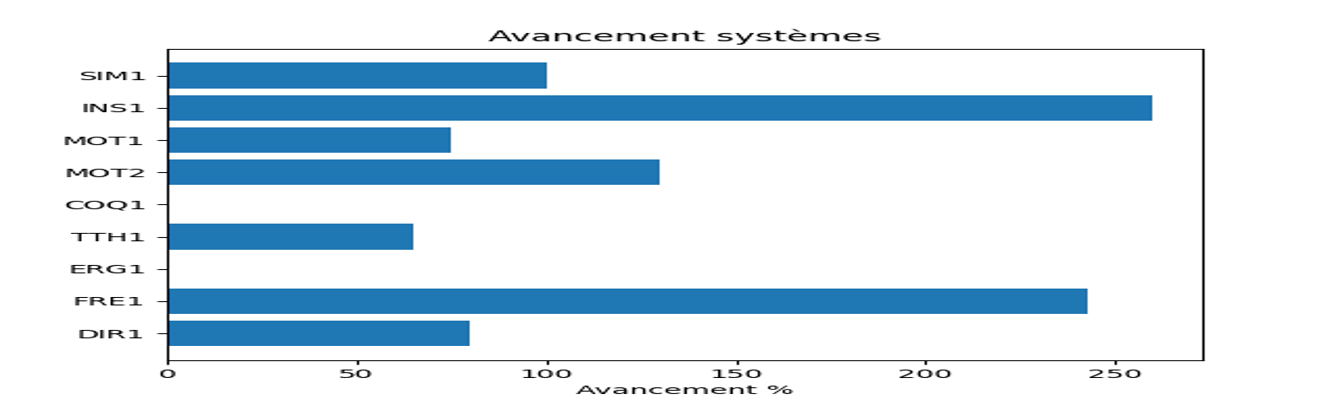
\includegraphics[width=1\linewidth]{img/progression_objectifs.png}}

\vspace{0.2cm} % spacing vertical

}

% this states the box starts at column 0 (edge of page), directly below the box labelled subtopic1 for a span of 1 (column wide)
\headerbox{Ordre du jour}{name=ordre_jour,column=0,below=objectif,span=1}{

\begin{itemize}
    \item \textbf{Rencontre gestion :}
    \begin{enumerate}
        \item Bons coups et mauvais coups
        \item Tour de table sur les avancements des objectifs
    \end{enumerate}
    \item \textbf{Rencontre technique :}
    \begin{enumerate}
        \item Question sur BMS monitoring
        \item Question sur algo de contrôle
        \item Question sur consommation télémétrie
    \end{enumerate}
\end{itemize}

\vspace{0.05cm} % spacing vertical
}

\headerbox{Membres}{name=membres,column=2,below=objectif_session,span=1}{
\vspace{0.3cm}


% inserts an image inside the box, 5 rows high | r = on the right along side text 
\begin{wrapfigure}[5]{r}{0.25\textwidth}
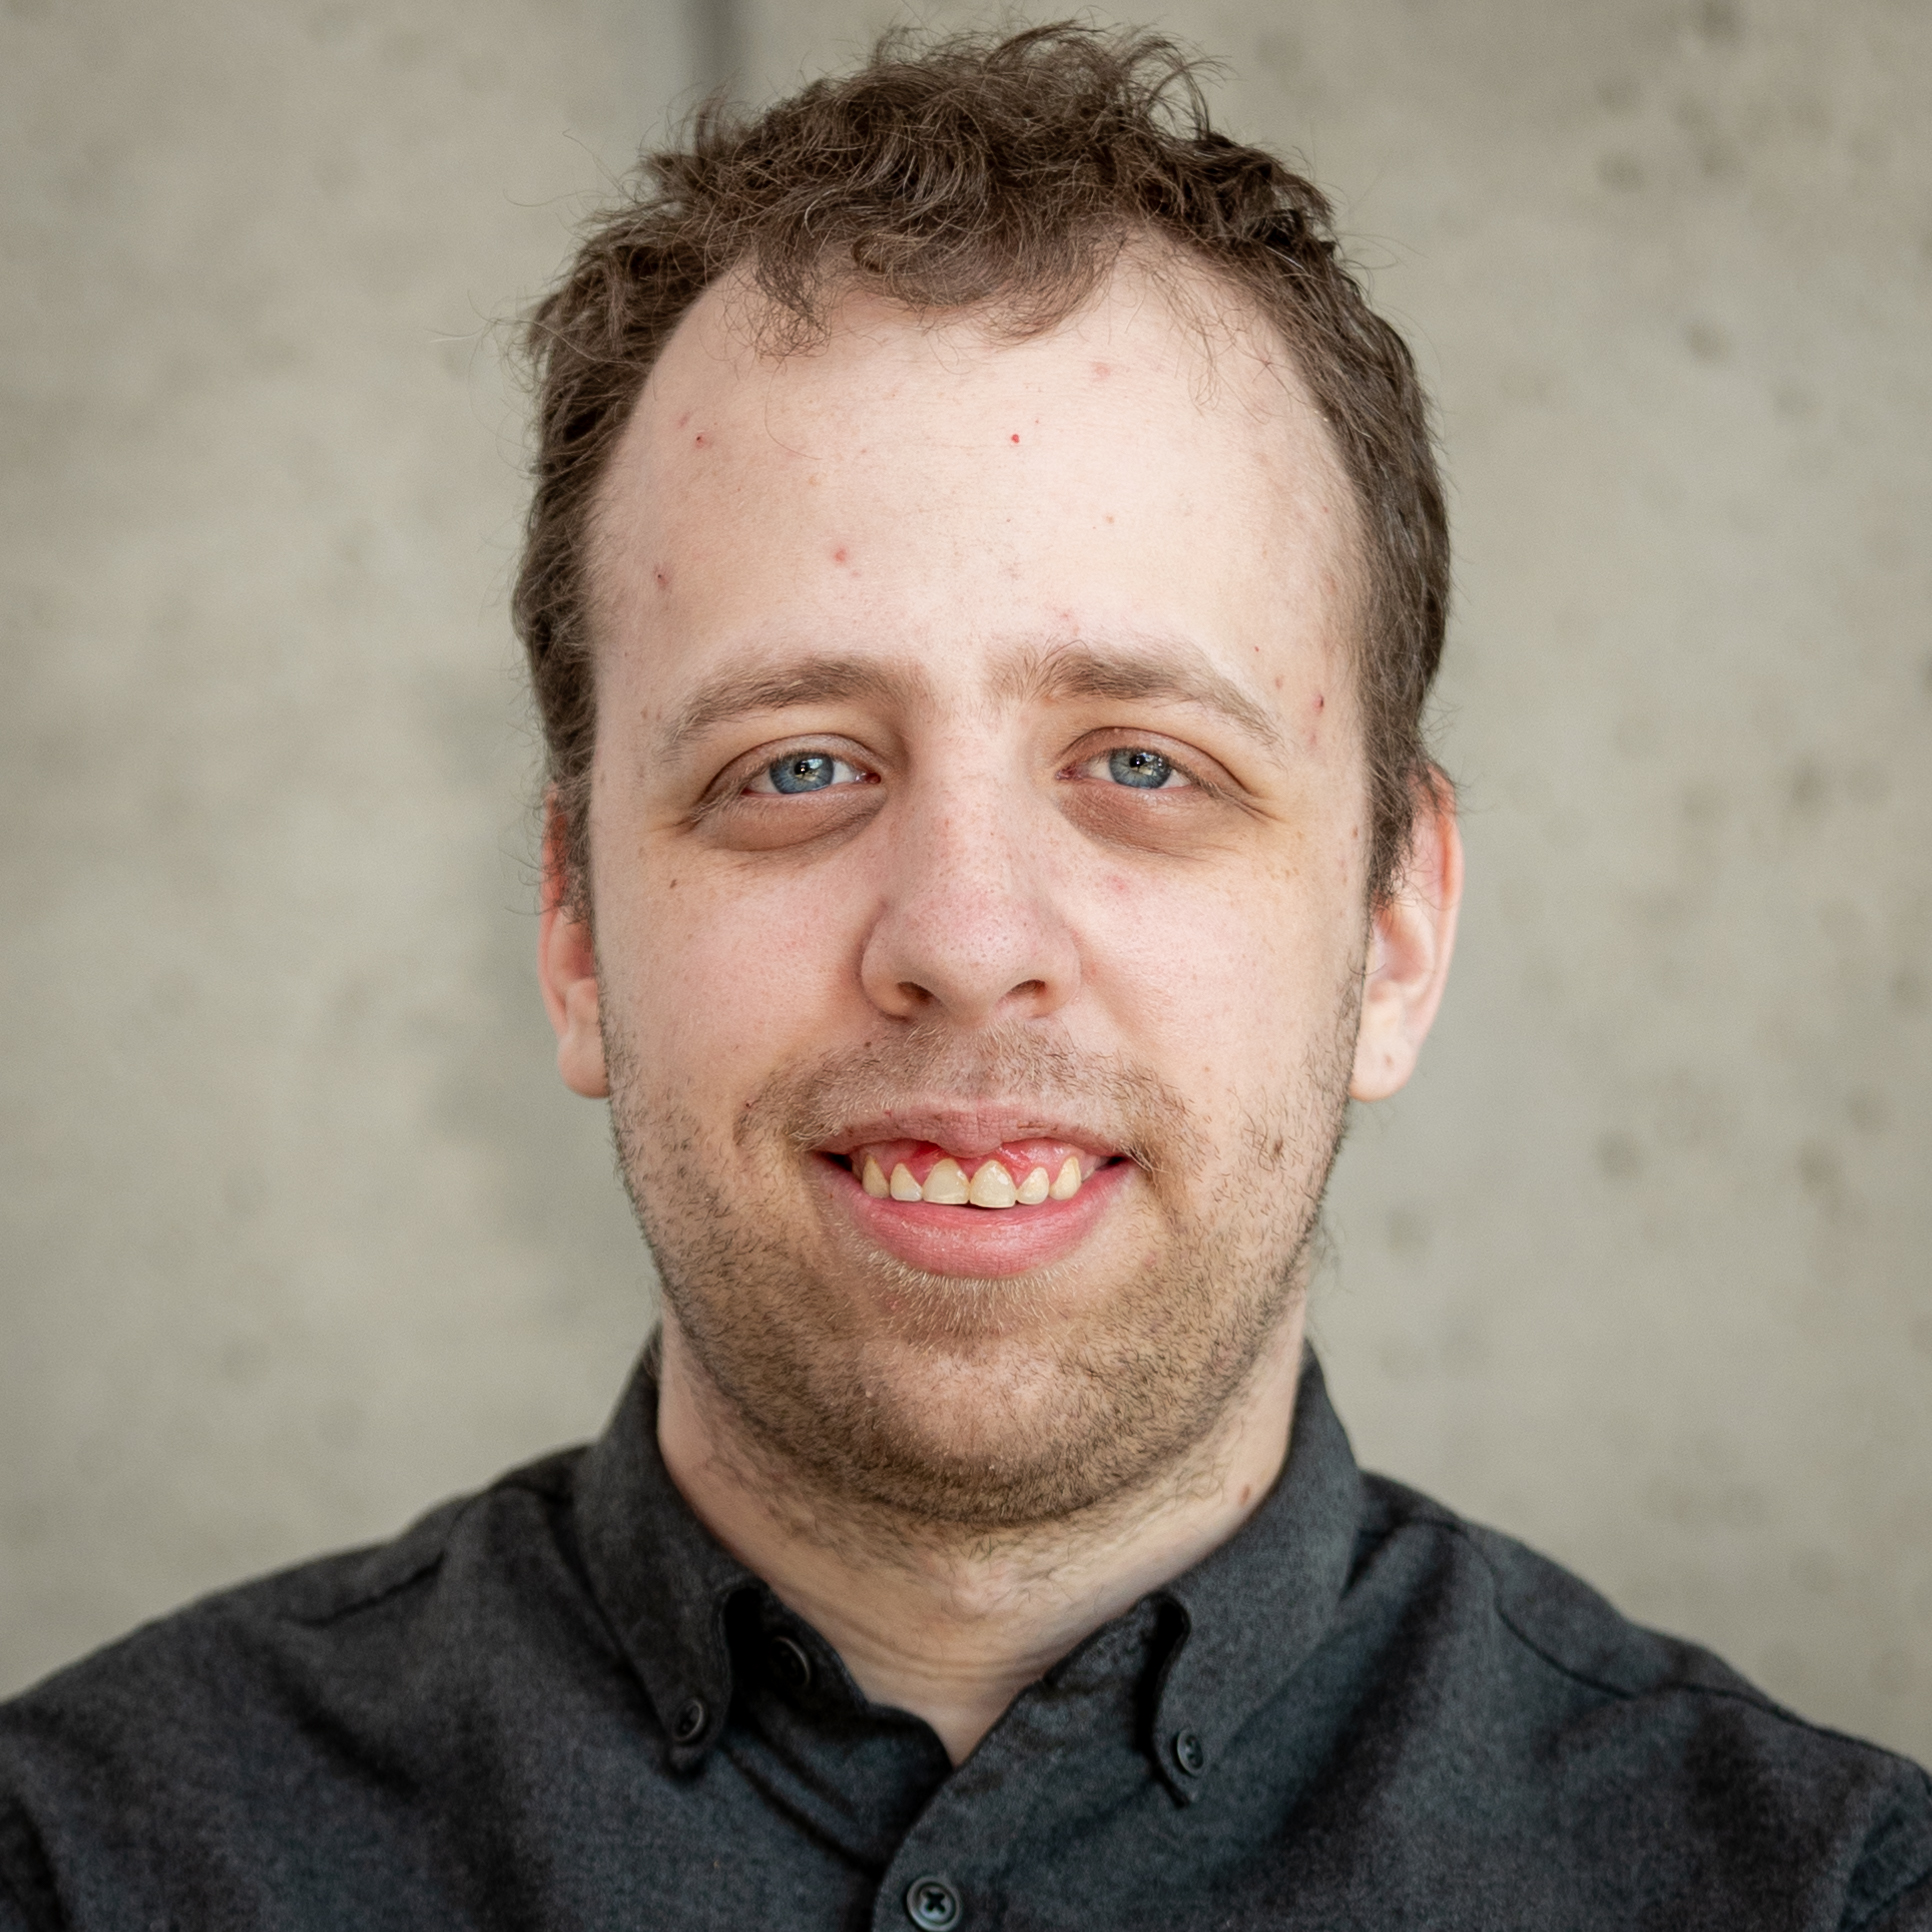
\includegraphics[width=0.9\linewidth]{img/membres/Alexandre-Bergeron-2.jpg} 
\end{wrapfigure}
\subsubsection*{}
\vspace{2mm}
\textbf{Alexandre Bergeron}


Télémétrie
\begin{wrapfigure}[5]{r}{0.25\textwidth}
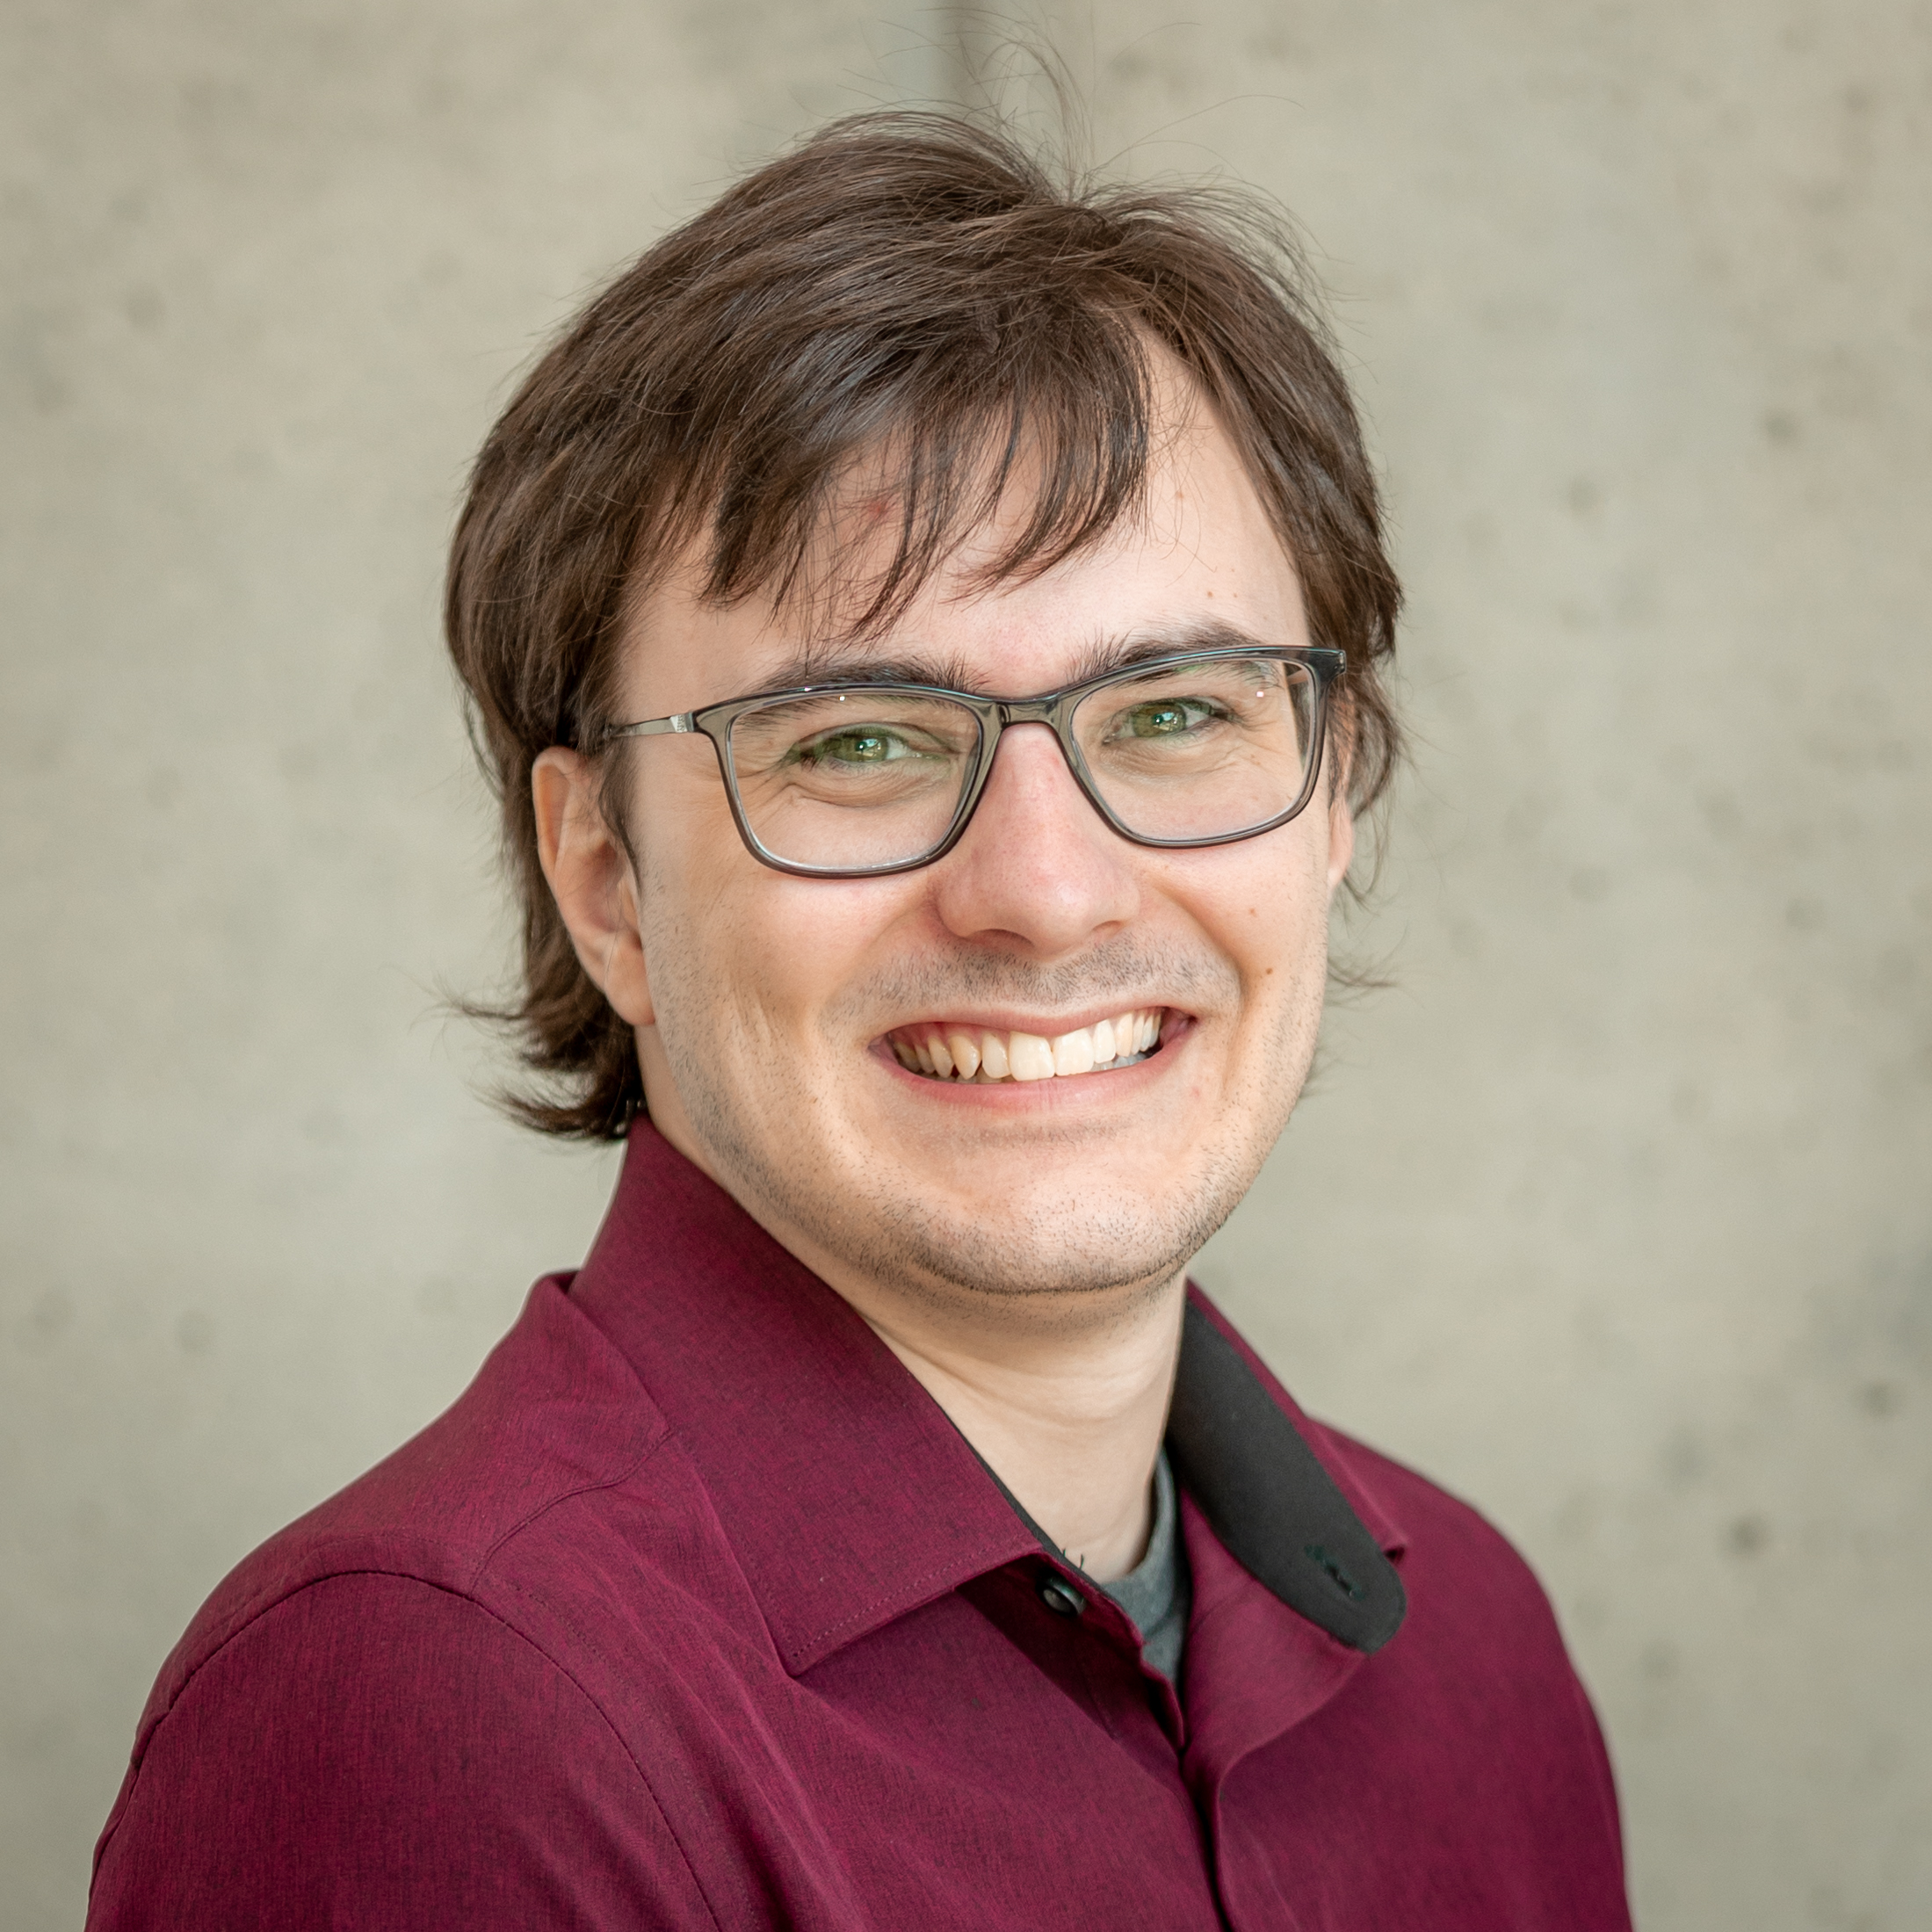
\includegraphics[width=.9\linewidth]{img/membres/Malik-Claveau-2.jpg} 
\end{wrapfigure}
\subsubsection*{}
\vspace{2mm}
\textbf{Malik Claveau}


Simulateur
\begin{wrapfigure}[5]{r}{0.25\textwidth}
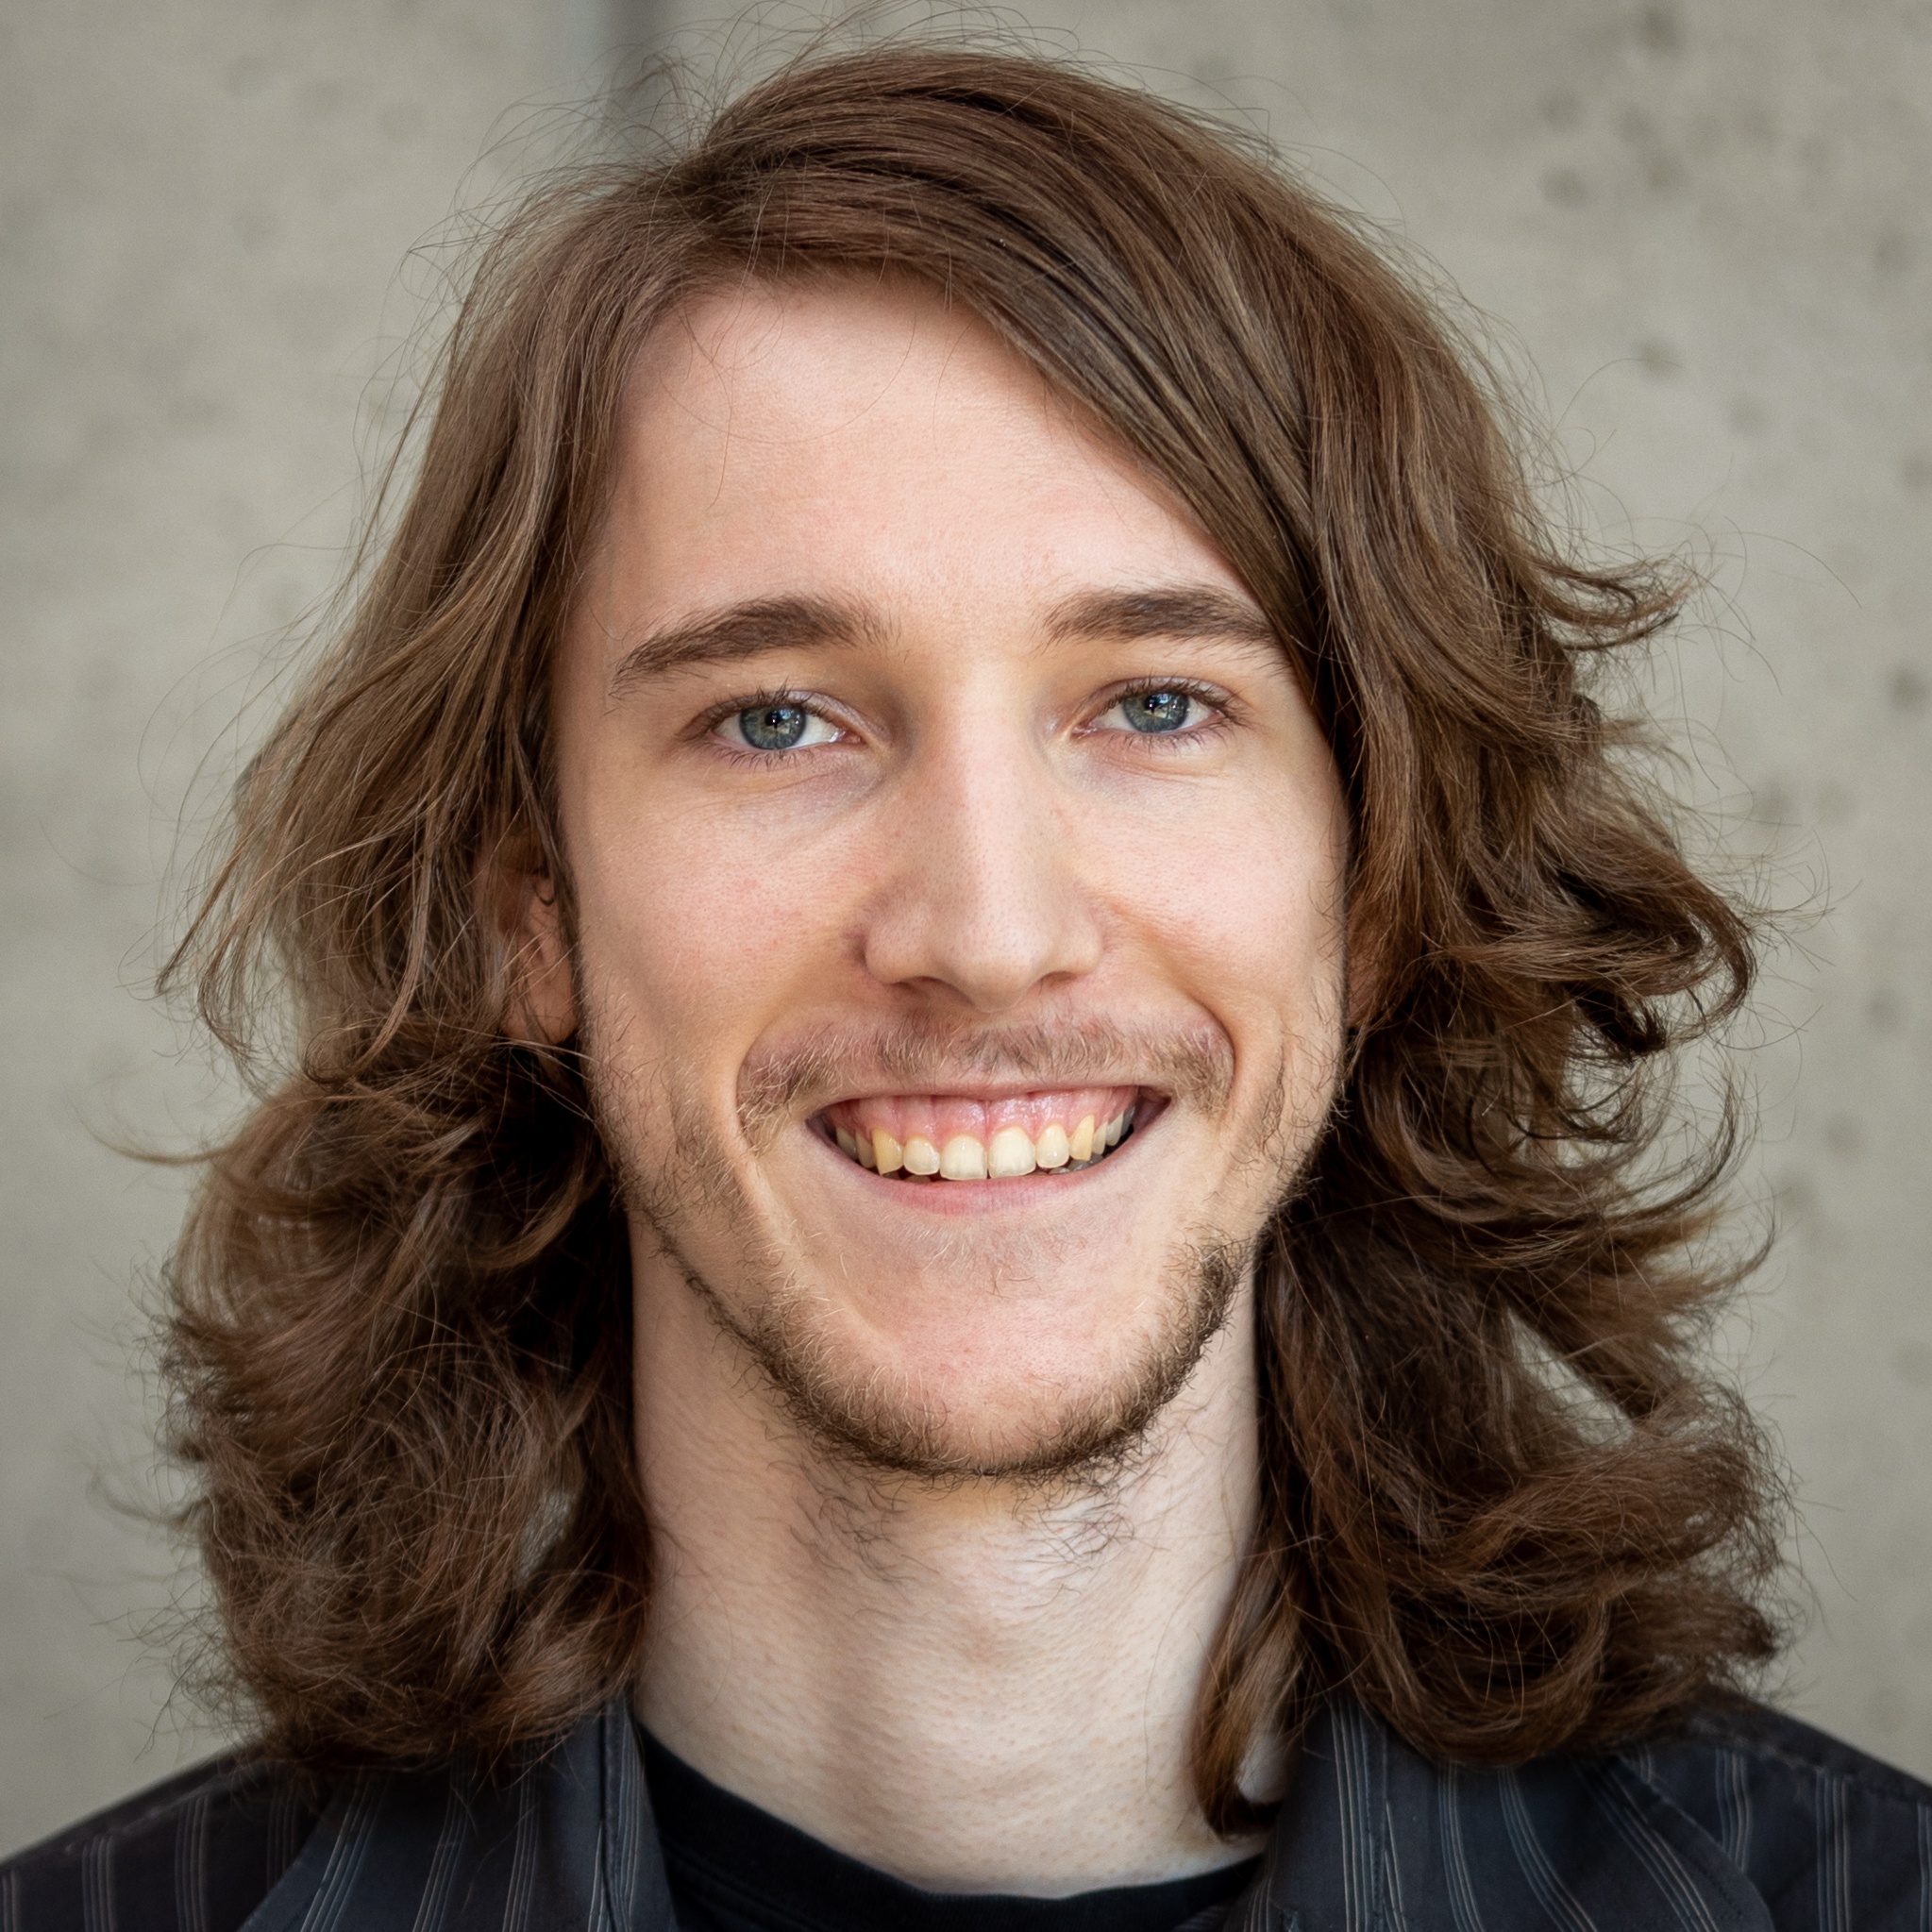
\includegraphics[width=.9\linewidth]{img/membres/Claude-Garrison-Pelletier-2.jpg} 
\end{wrapfigure}
\subsubsection*{}
\vspace{2mm}
\textbf{Claude Garrison-Pelletier}


Simulateur
\begin{wrapfigure}[5]{r}{0.25\textwidth}
\includegraphics[width=.9\linewidth]{img/membres/Charles-Étienne-Granger-3.jpg} 
\end{wrapfigure}
\subsubsection*{}
\vspace{2mm}
\textbf{Charles-Étienne Granger}


Télémétrie
\begin{wrapfigure}[5]{r}{0.25\textwidth}
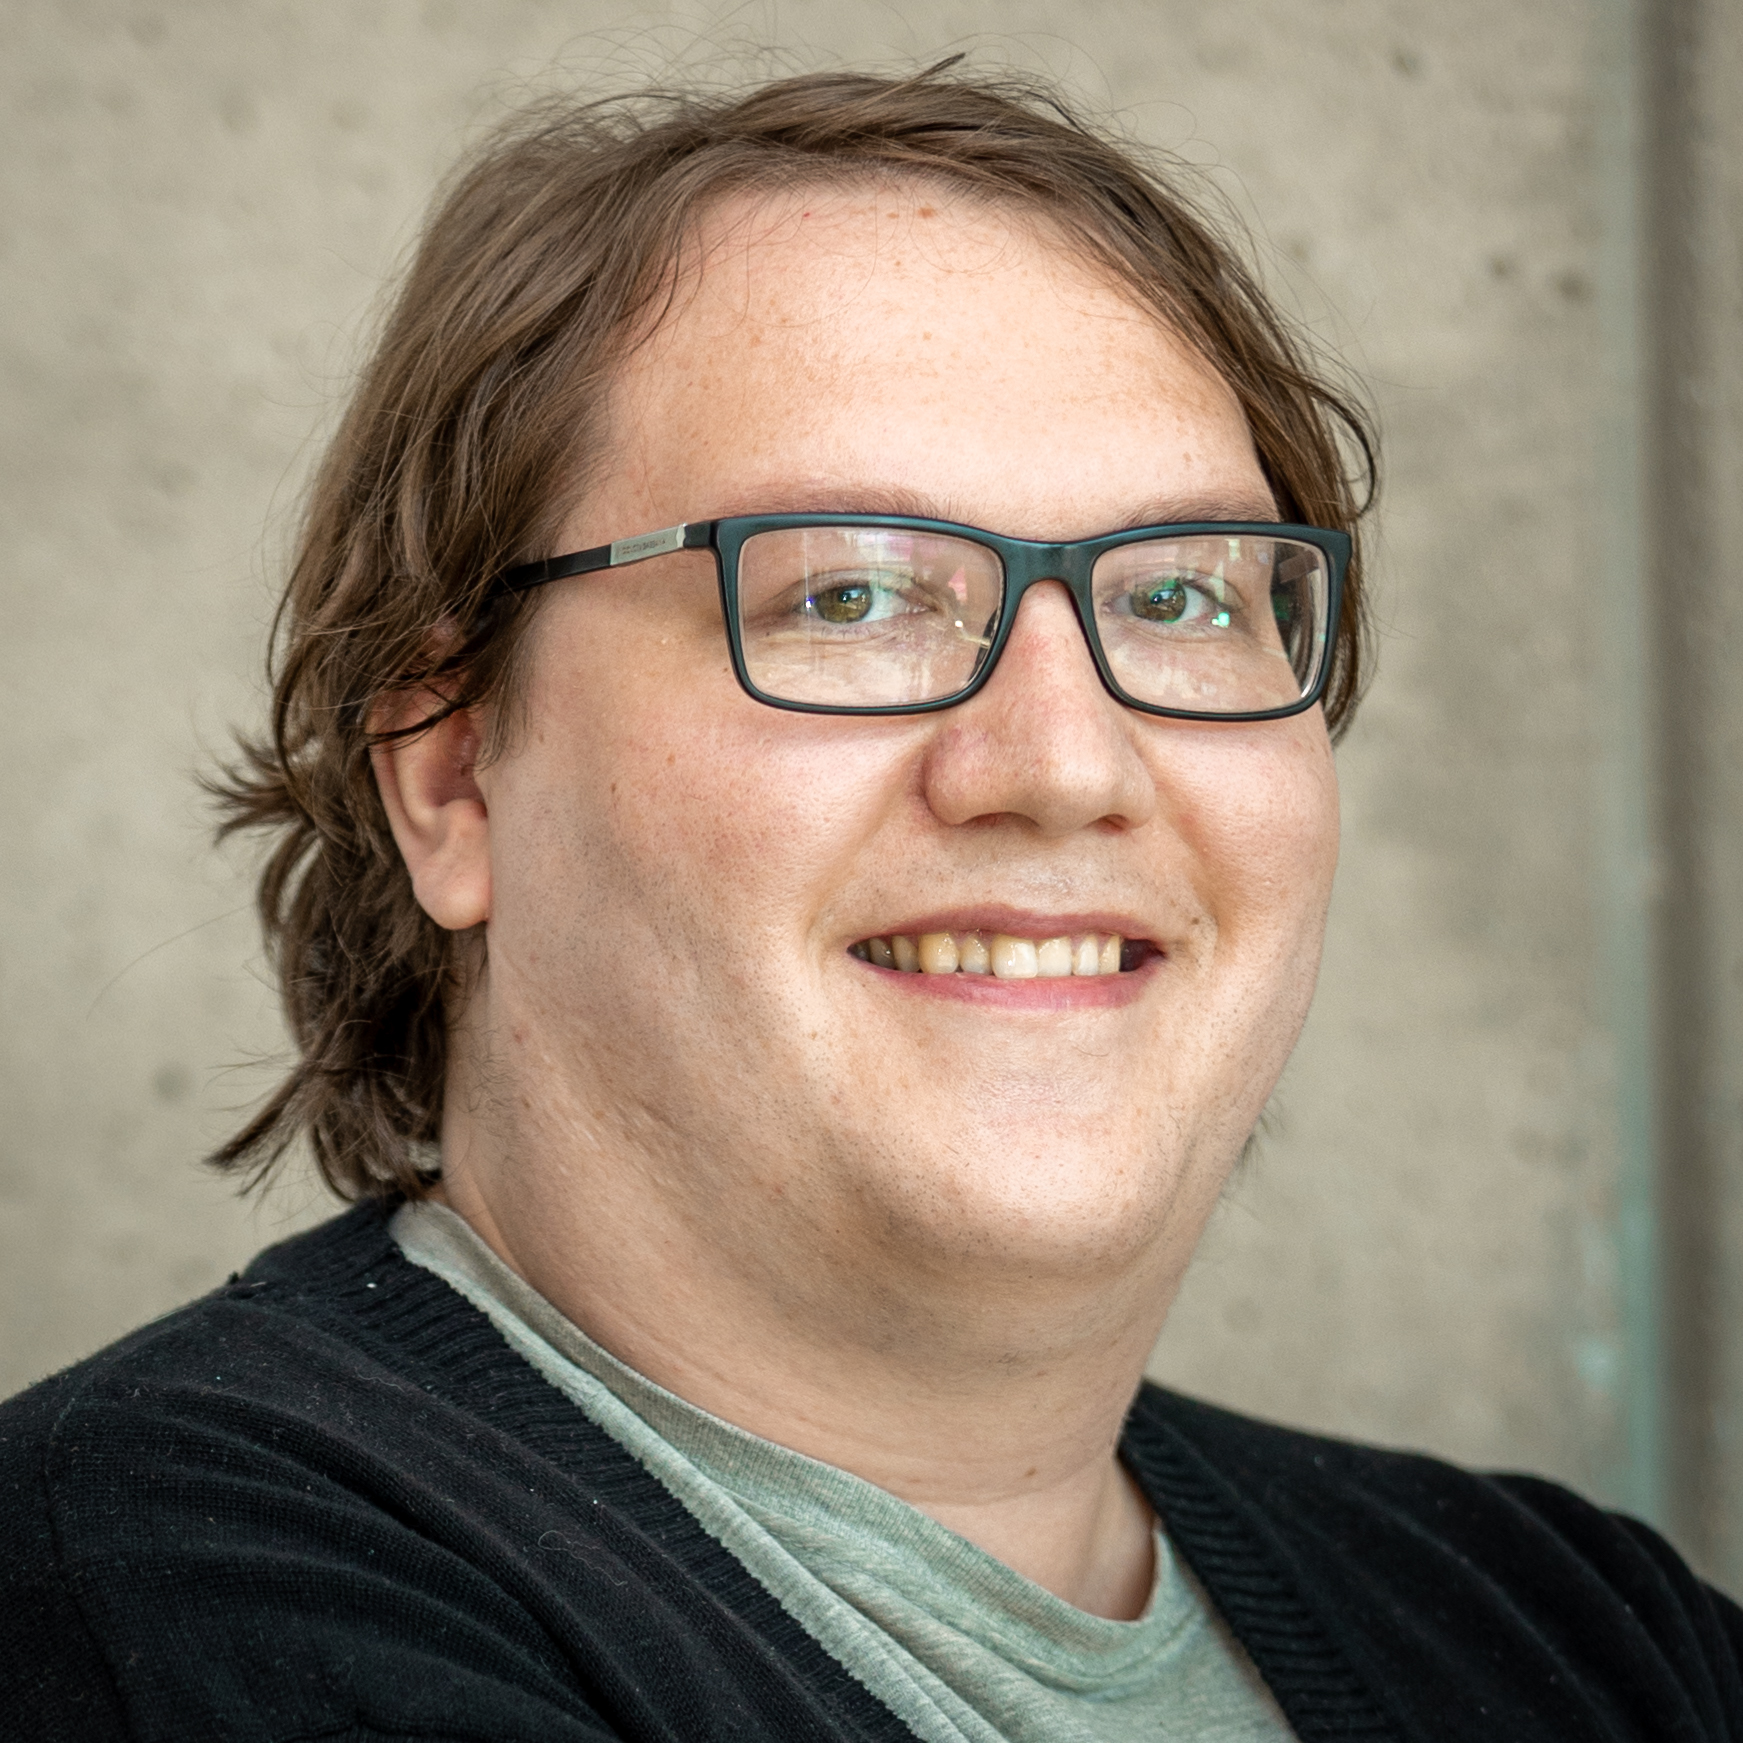
\includegraphics[width=.9\linewidth]{img/membres/Marian-Lambert-Rivest-3.jpg} 
\end{wrapfigure}
\subsubsection*{}
\vspace{2mm}
\textbf{Marian Lambert-Rivest}


Simulateur
\begin{wrapfigure}[5]{r}{0.25\textwidth}
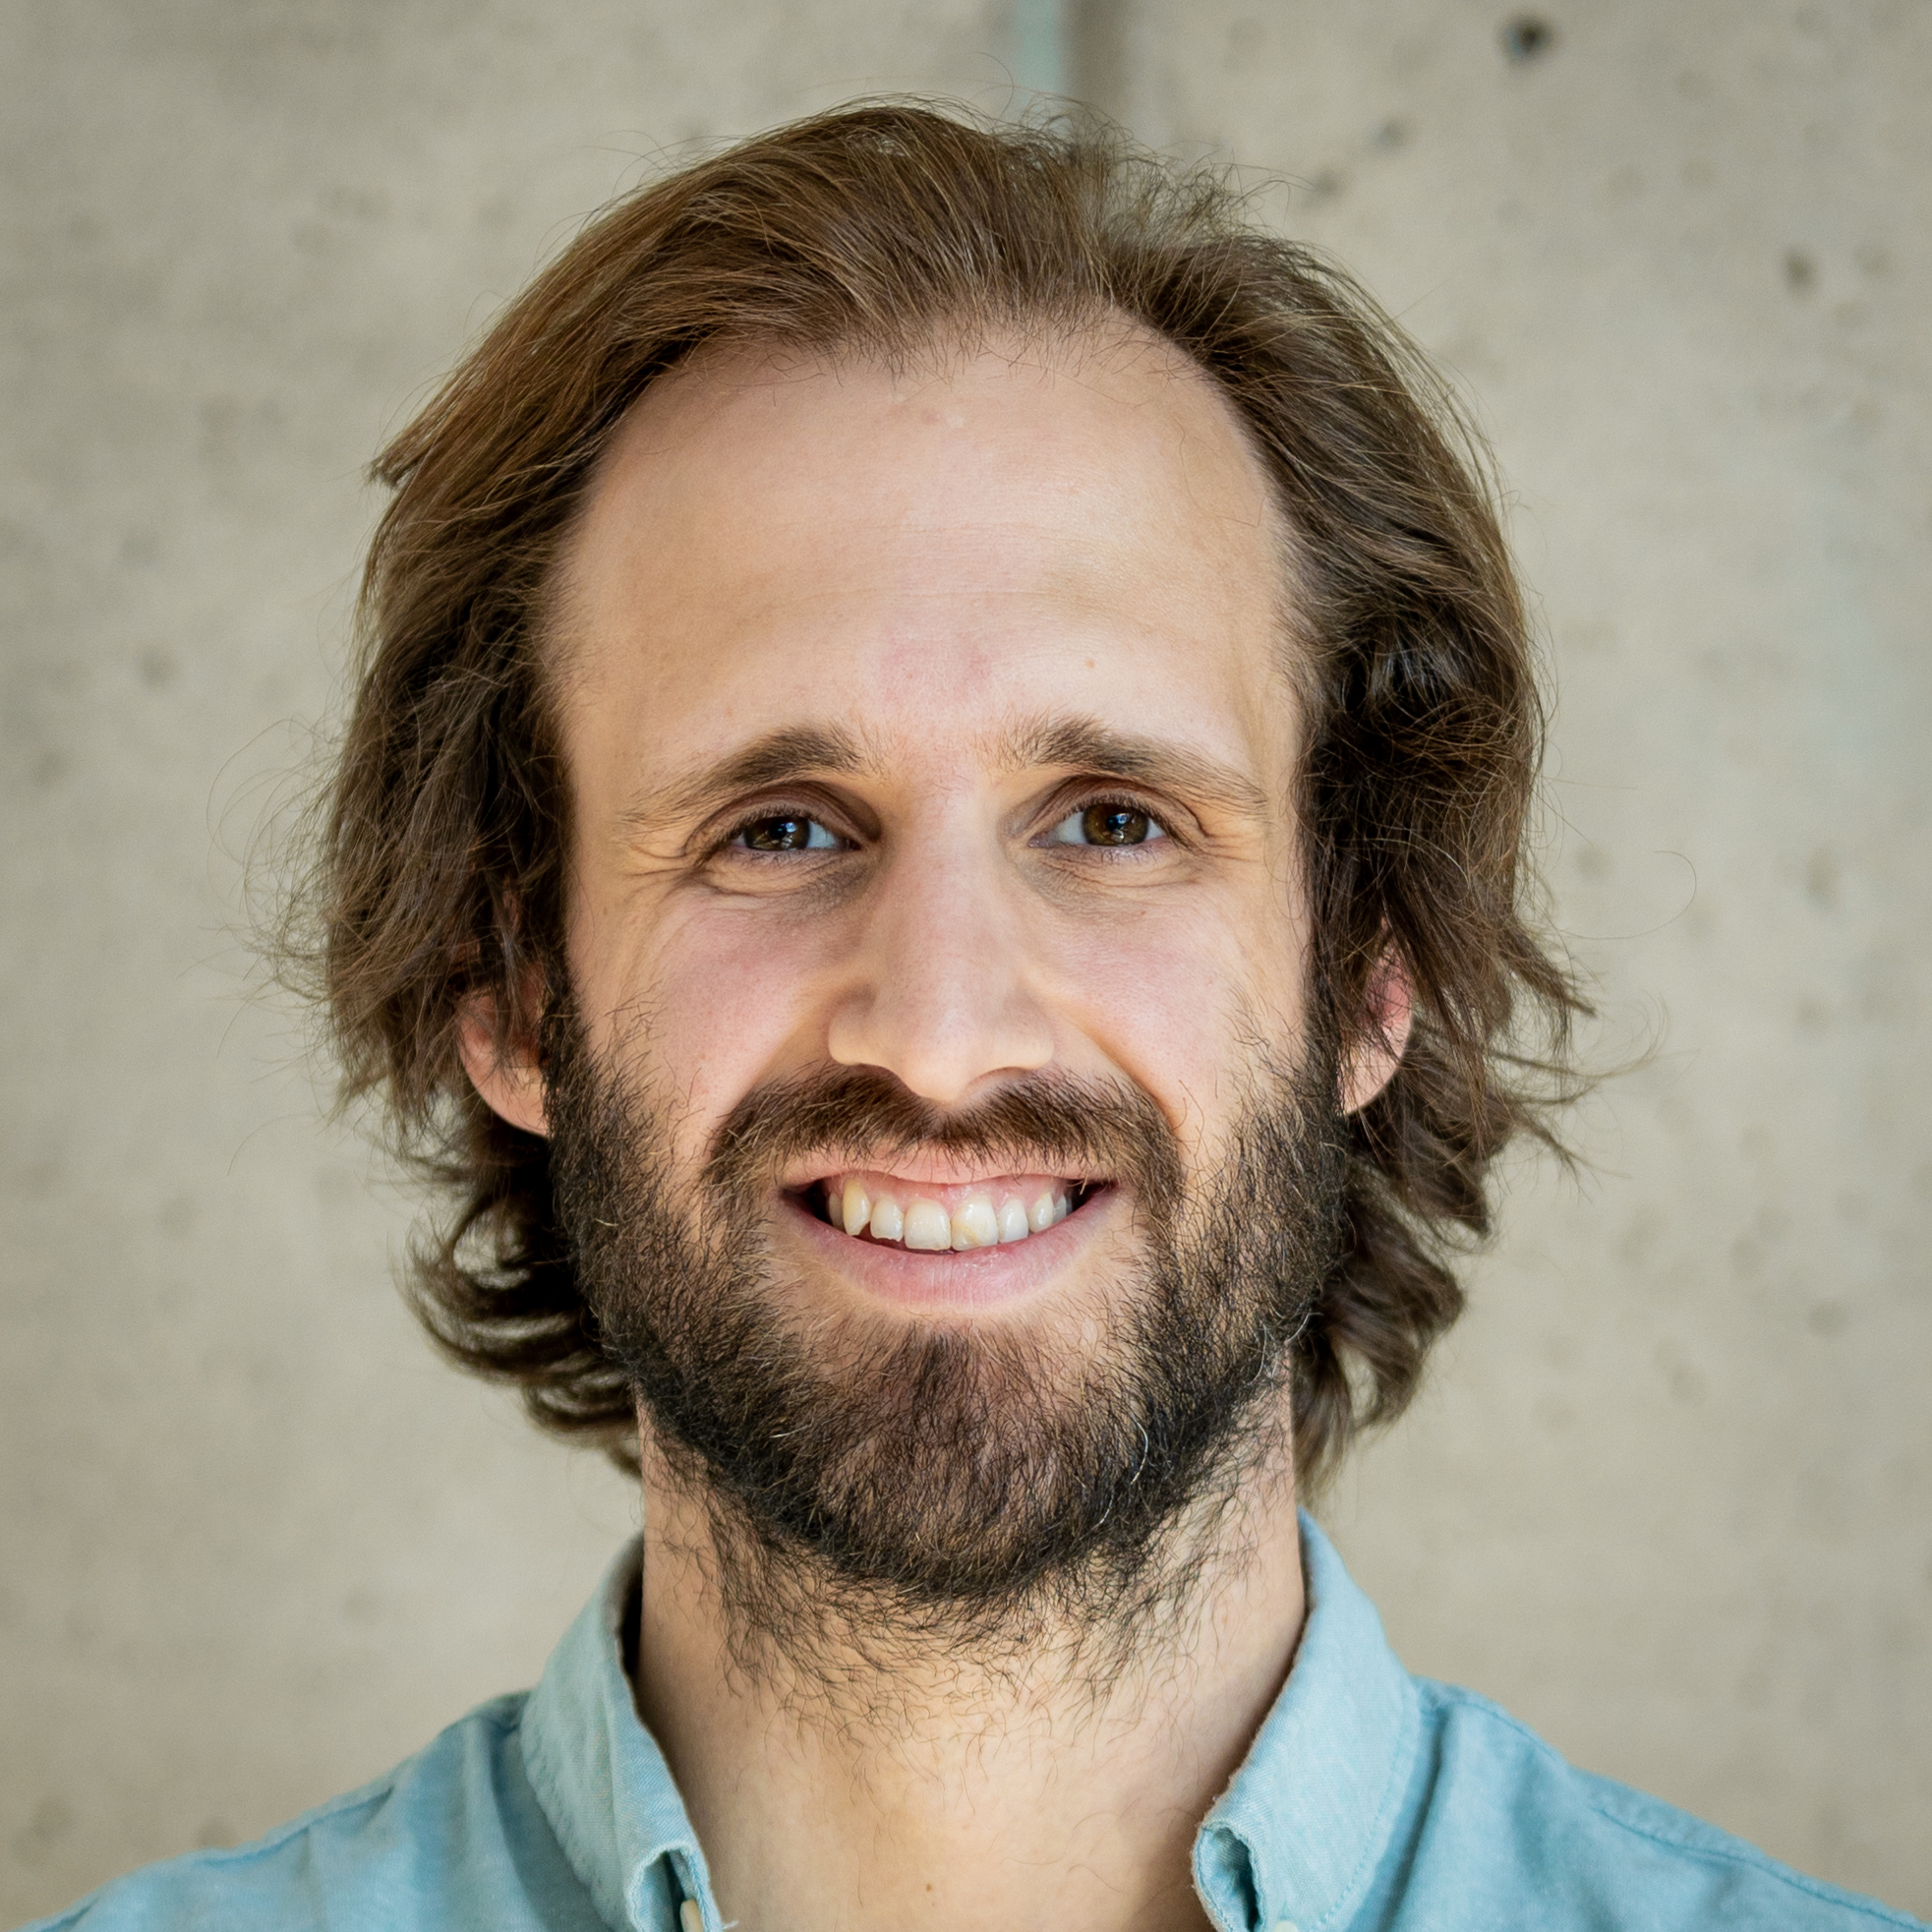
\includegraphics[width=.9\linewidth]{img/membres/Mathieu-Parent-2.jpg} 
\end{wrapfigure}
\subsubsection*{}
\vspace{2mm}
\textbf{Mathieu Parent}


Télémétrie
\begin{wrapfigure}[5]{r}{0.25\textwidth}
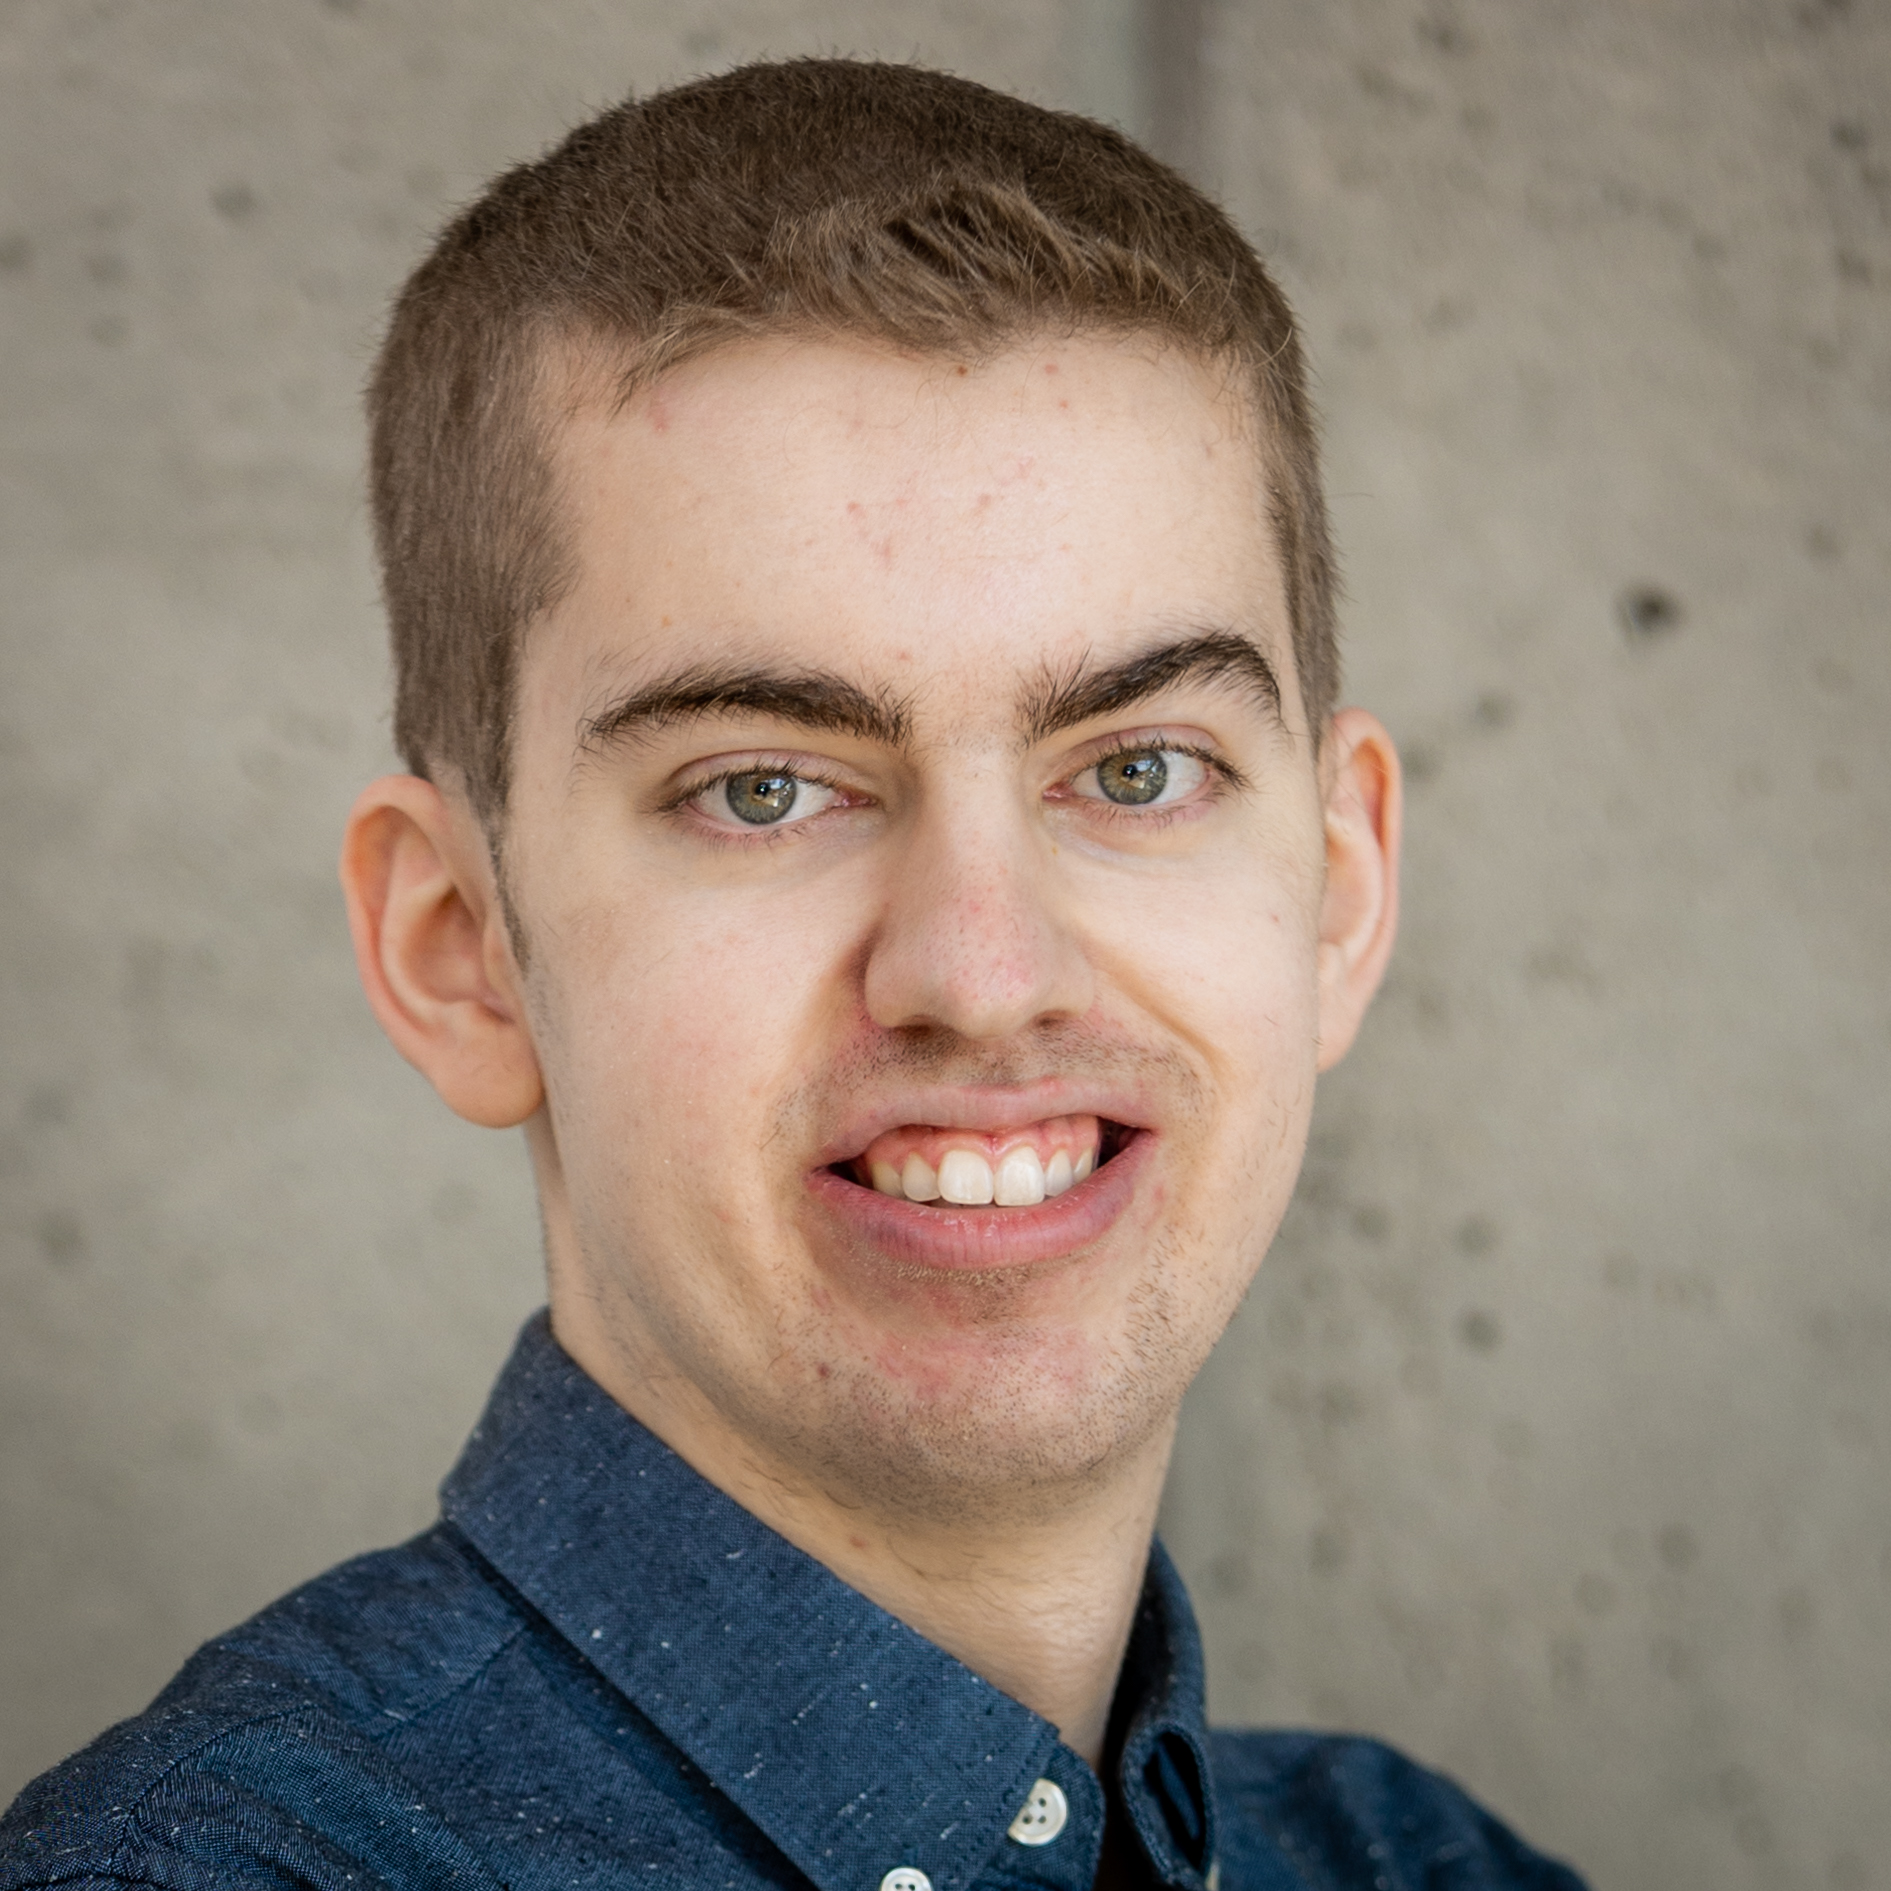
\includegraphics[width=.9\linewidth]{img/membres/Gabriel-Quirion-3.jpg} 
\end{wrapfigure}
\subsubsection*{}
\vspace{2mm}
\textbf{Gabriel Quirion}


Contrôle
\begin{wrapfigure}[5]{r}{0.25\textwidth}
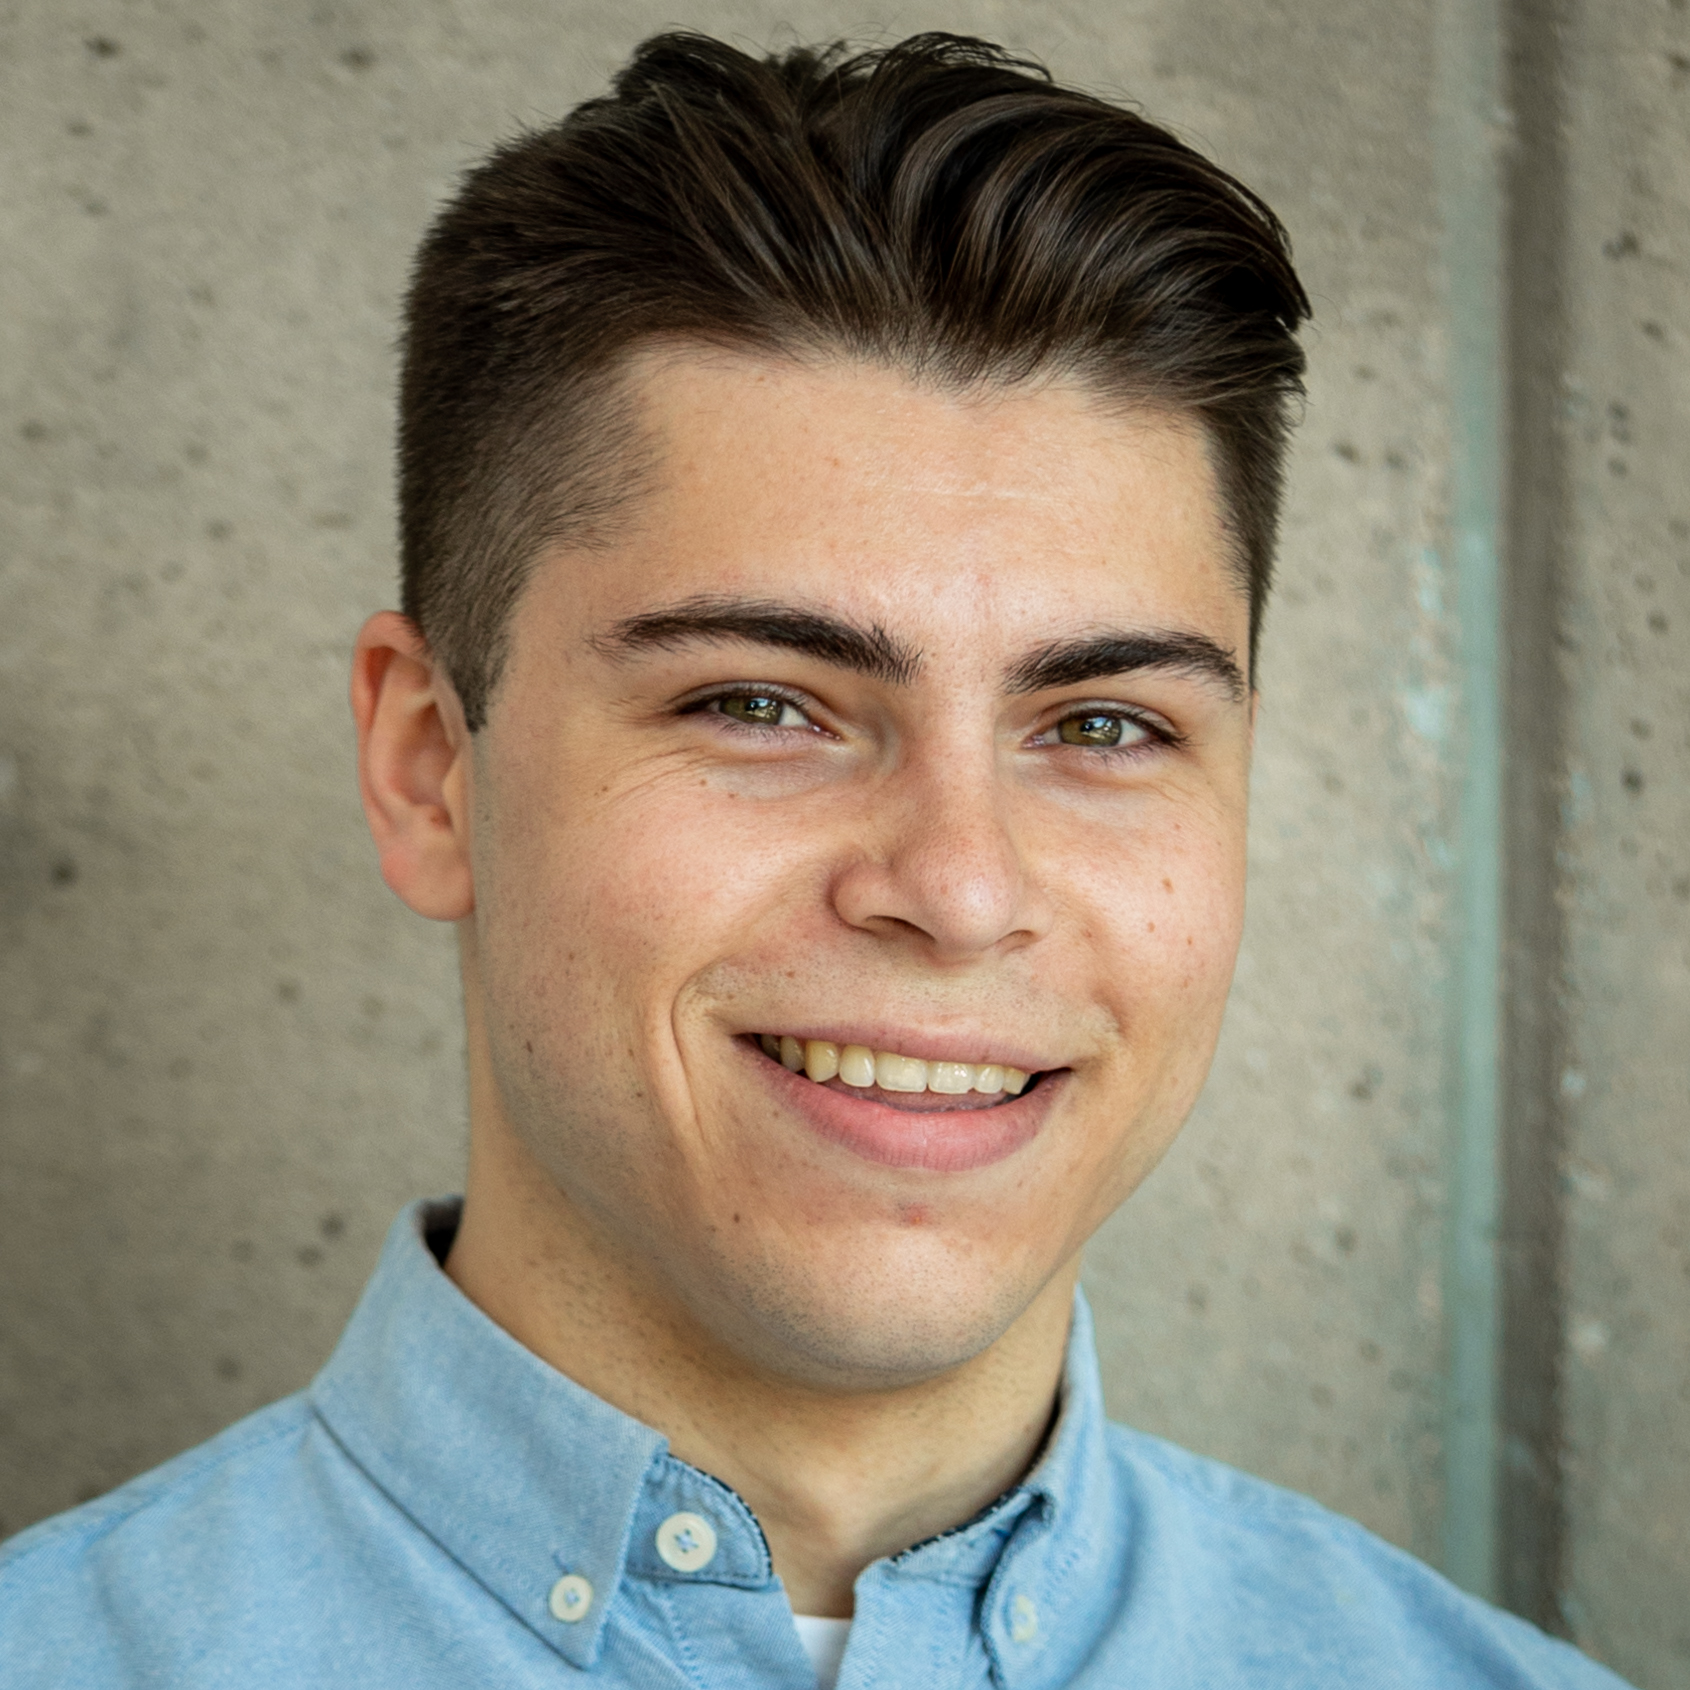
\includegraphics[width=.9\linewidth]{img/membres/William-Rousseau-2.jpg} 
\end{wrapfigure}
\subsubsection*{}
\vspace{2mm}
\textbf{William Rousseau}


Télémétrie
\begin{wrapfigure}[5]{r}{0.25\textwidth}
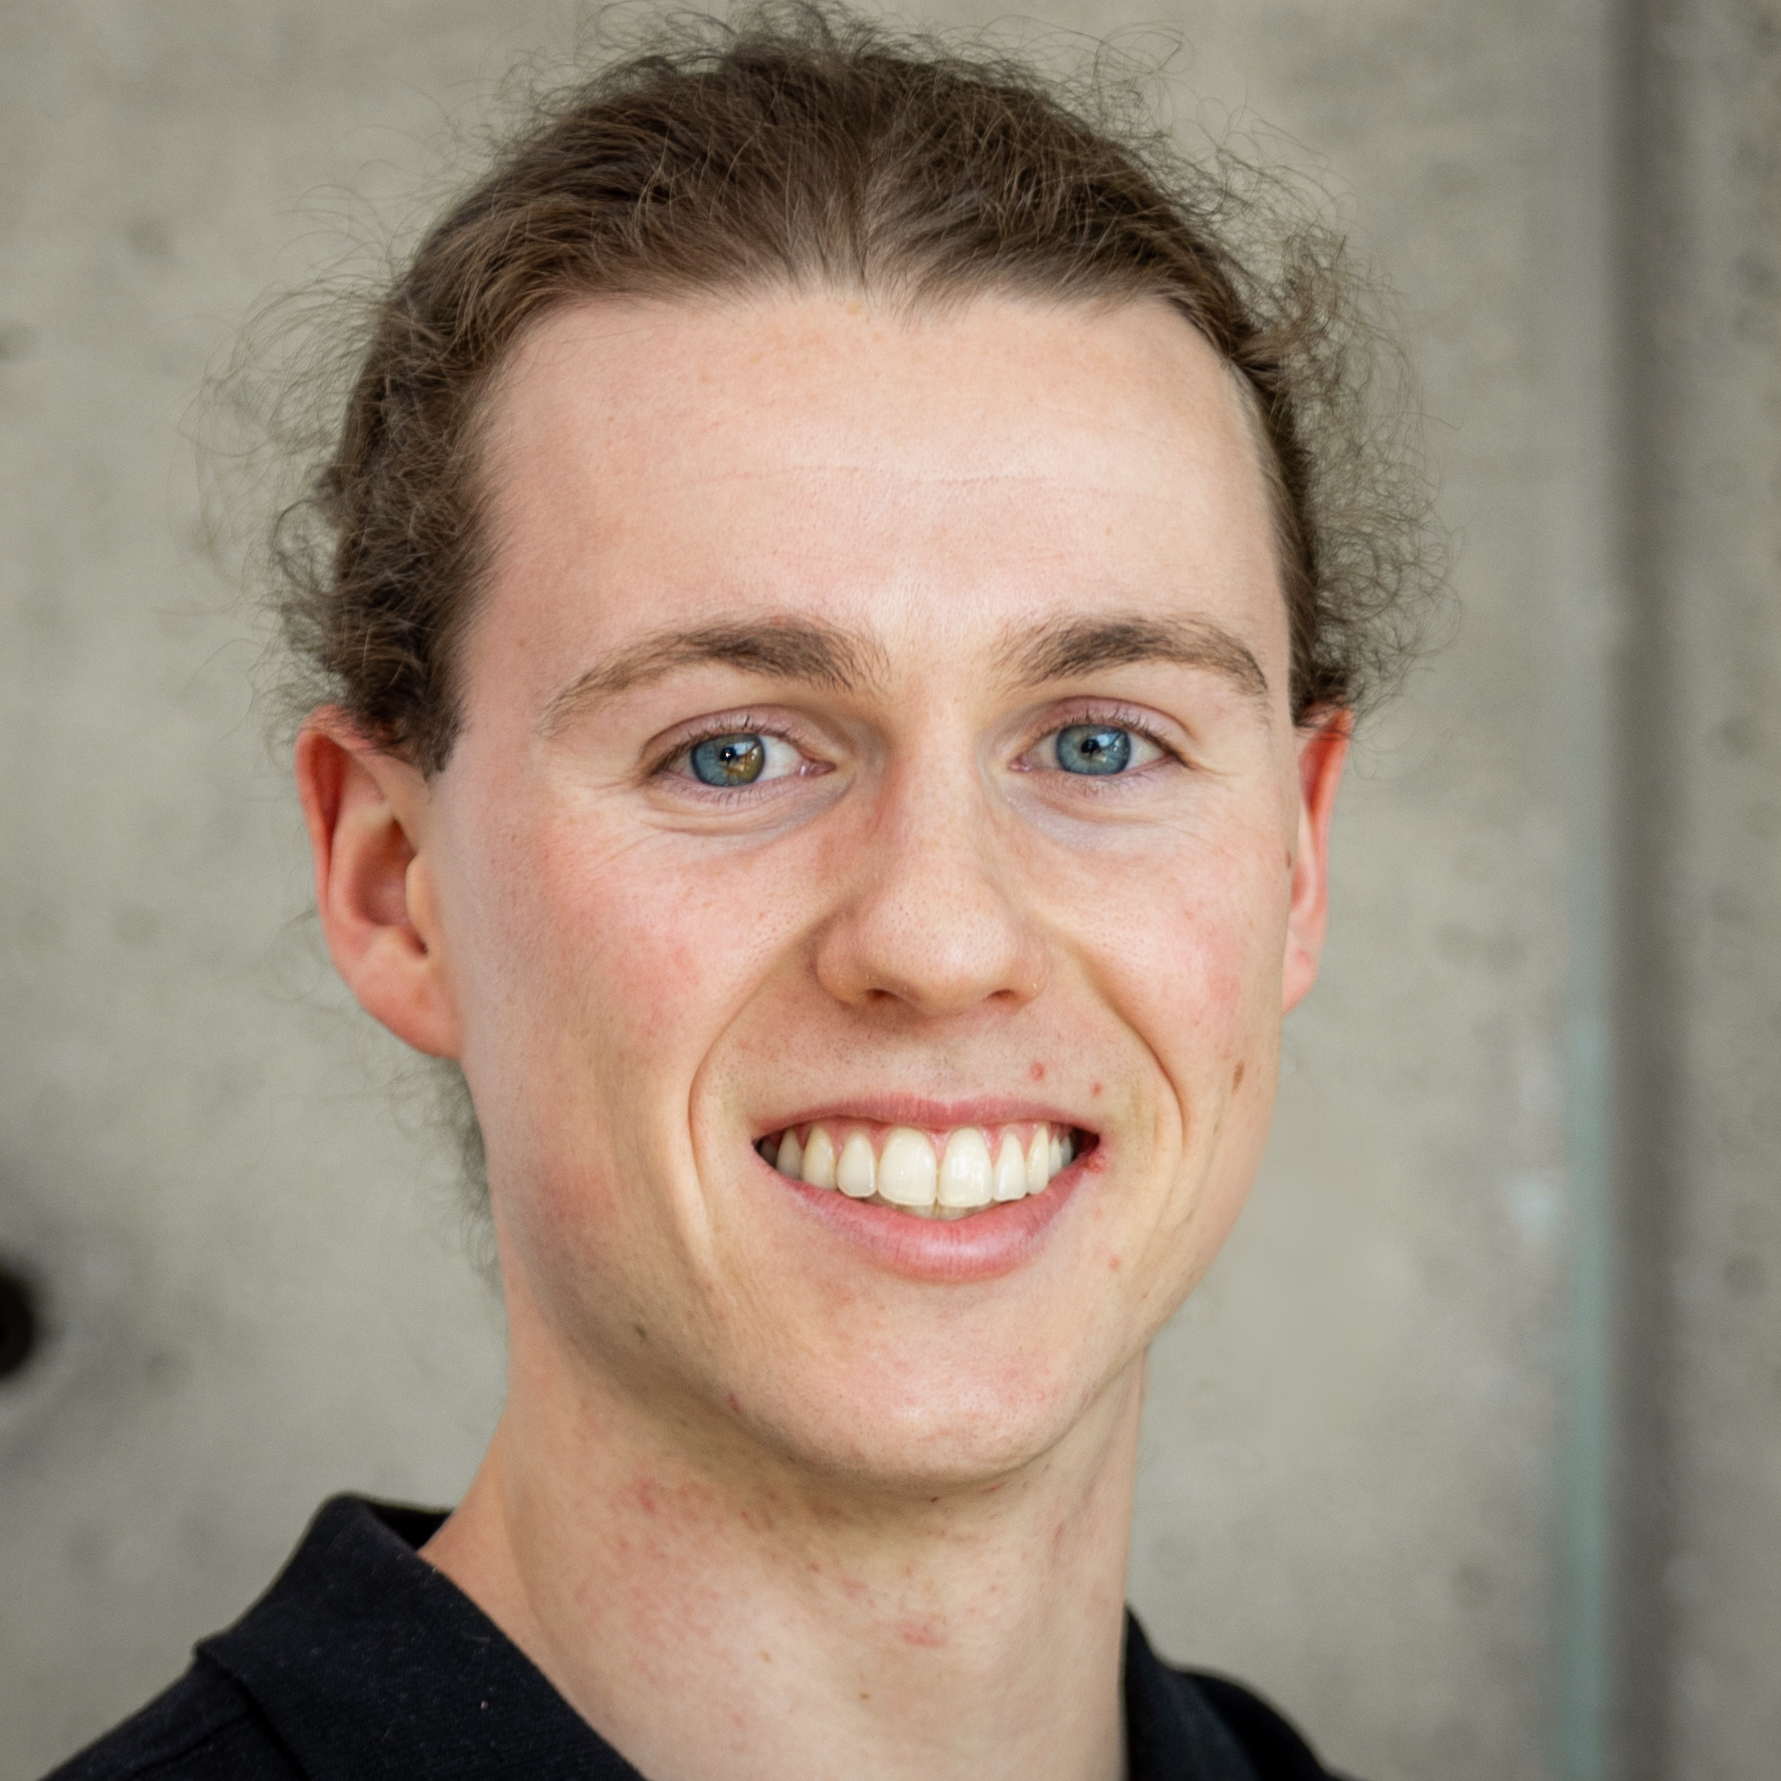
\includegraphics[width=.9\linewidth]{img/membres/Louis-Tardif-3.jpg} 
\end{wrapfigure}
\subsubsection*{}
\vspace{2mm}
\textbf{Louis Tardif}


Contrôle
\vspace{1cm}
%\begin{wrapfigure}[8]{r}{0.25\textwidth}
%\includegraphics[width=.9\linewidth]{DevOps.png} 
%\includegraphics[width=.9\linewidth]{DevOps.png} 
%\end{wrapfigure}
%
%\vspace{0.3cm}
%\subsubsection*{2. Another sub section:}
%
%Subsection description
%
%\vspace{2.3cm} %remove this, only added for spacing
%
%\begin{wrapfigure}[5]{r}{0.25\textwidth}
%\includegraphics[width=.9\linewidth]{TUDublin.jpg} 
%\end{wrapfigure}
%
%\vspace{0.35cm}
%\subsubsection*{3. Another sub section:}
%Final Subsection description
%
%\vspace{2cm} %remove this, only added for spacing
}


\headerbox{Courbe en S}{name=courbe_s,column=0,span=2,below=ordre_jour}{
{
    {
        \hspace{1cm}
        \centering
    	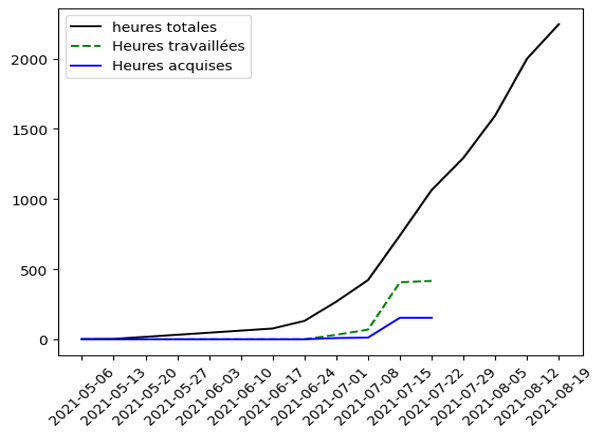
\includegraphics[scale=.54]{img/Courbe_S.png}
    }
}

}

\headerbox{Heures travaillées}{name=heures,column=0,span=2,below=courbe_s}{
{
    
    {
        \hspace{1cm}
        \centering
    	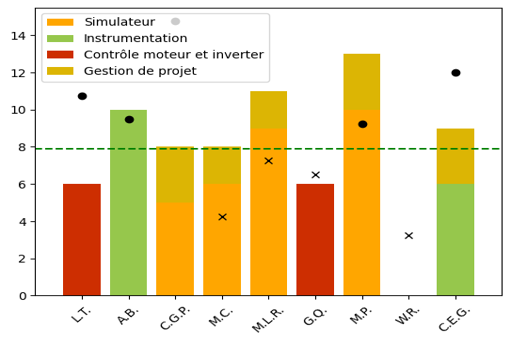
\includegraphics[scale=.75]{img/heures_travaillees.png}
    }
    \vspace{1.3cm}
}

}

\end{poster}

\begin{poster}
{
grid=false,
headerborder=open, % Adds a border around the header of content boxes
colspacing=1em, % Column spacing
bgColorOne=white, % Background color for the gradient on the left side of the poster
bgColorTwo=white, % Background color for the gradient on the right side of the poster
borderColor=Mycolor1, % Border color
headerColorOne=Mycolor2, % Background color for the header in the content boxes (left side)
headerColorTwo=Mycolor2, % Background color for the header in the content boxes (right side)
headerFontColor=white, % Text color for the header text in the content boxes
boxColorOne=white, % Background color of the content boxes
textborder=rounded, %rectangle, % Format of the border around content boxes, can be: none, bars, coils, triangles, rectangle, rounded, roundedsmall, roundedright or faded
eyecatcher=false, % Set to false for ignoring the left logo in the title and move the title left
headerheight=0\textheight, % Height of the header
headershape=rounded, % Specify the rounded corner in the content box headers, can be: rectangle, small-rounded, roundedright, roundedleft or rounded
headershade=plain,
headerfont=\Large\textsf, % Large, bold and sans serif font in the headers of content boxes
%textfont={\setlength{\parindent}{1.5em}}, % Uncomment for paragraph indentation
linewidth=1pt % Width of the border lines around content boxes
}
{}
{\textsf{{}}} % Titre vide pcq sinon ça plante


% this states the box starts at column 0 (edge of page), row 0 (top of page) for a span of 3 (columns wide)
\headerbox{Tâches accomplies}{name=taches,column=0,row=0, span=3}{
%{\begin{tabularx}{\linewidth}{
    |>{\hsize=2.5\hsize}X|% 10% of 4\hsize 
    >{\hsize=0.5\hsize}X|% 30% of 4\hsize
    >{\hsize=0.75\hsize}X|% 30% of 4\hsize 
    >{\hsize=0.25\hsize}X|% 30% of 4\hsize 
       % sum=0.2\hsize for 4 columns
  }
    \hline
    \textbf{Objectif} & \textbf{Système} & \textbf{Responsable} & \textbf{Heures}\\\hline
    Mise en place serveur et VPN & Transferts Thermiques & Charles-Etienne Granger & 9.0\\\hline
    Automatiser la mise à jour des tables et graphiques. & Gestion de projet & Charles-Etienne Granger & 19.0\\\hline
  \end{tabularx}
     }
\centering
{\begin{tabularx}{\linewidth}{
    |>{\hsize=2.5\hsize}X|% 10% of 4\hsize 
    >{\hsize=0.5\hsize}X|% 30% of 4\hsize
    >{\hsize=0.75\hsize}X|% 30% of 4\hsize 
    >{\hsize=0.25\hsize}X|% 30% of 4\hsize 
       % sum=0.2\hsize for 4 columns
  }
    \hline
    \textbf{Objectif} & \textbf{Système} & \textbf{Responsable} & \textbf{Heures}\\\hline
    Mise en place serveur et VPN & Transferts Thermiques & Charles-Etienne Granger & 9.0\\\hline
    Automatiser la mise à jour des tables et graphiques. & Gestion de projet & Charles-Etienne Granger & 19.0\\\hline
  \end{tabularx}
     }

\vspace{0.2cm} % spacing vertical

%\vspace{2cm} %remove this, only added for spacing

}

% this states the box starts at column 0 (edge of page), directly below the box labelled introduction for a span of 1 (column wide)
\headerbox{Avancement systèmes}{name=systemes,column=1,below=taches,span=2}{

%\vspace{0.15cm}
\textit{AVANCEMENT DES SYSTÈMES DU PROJET}
\centering
{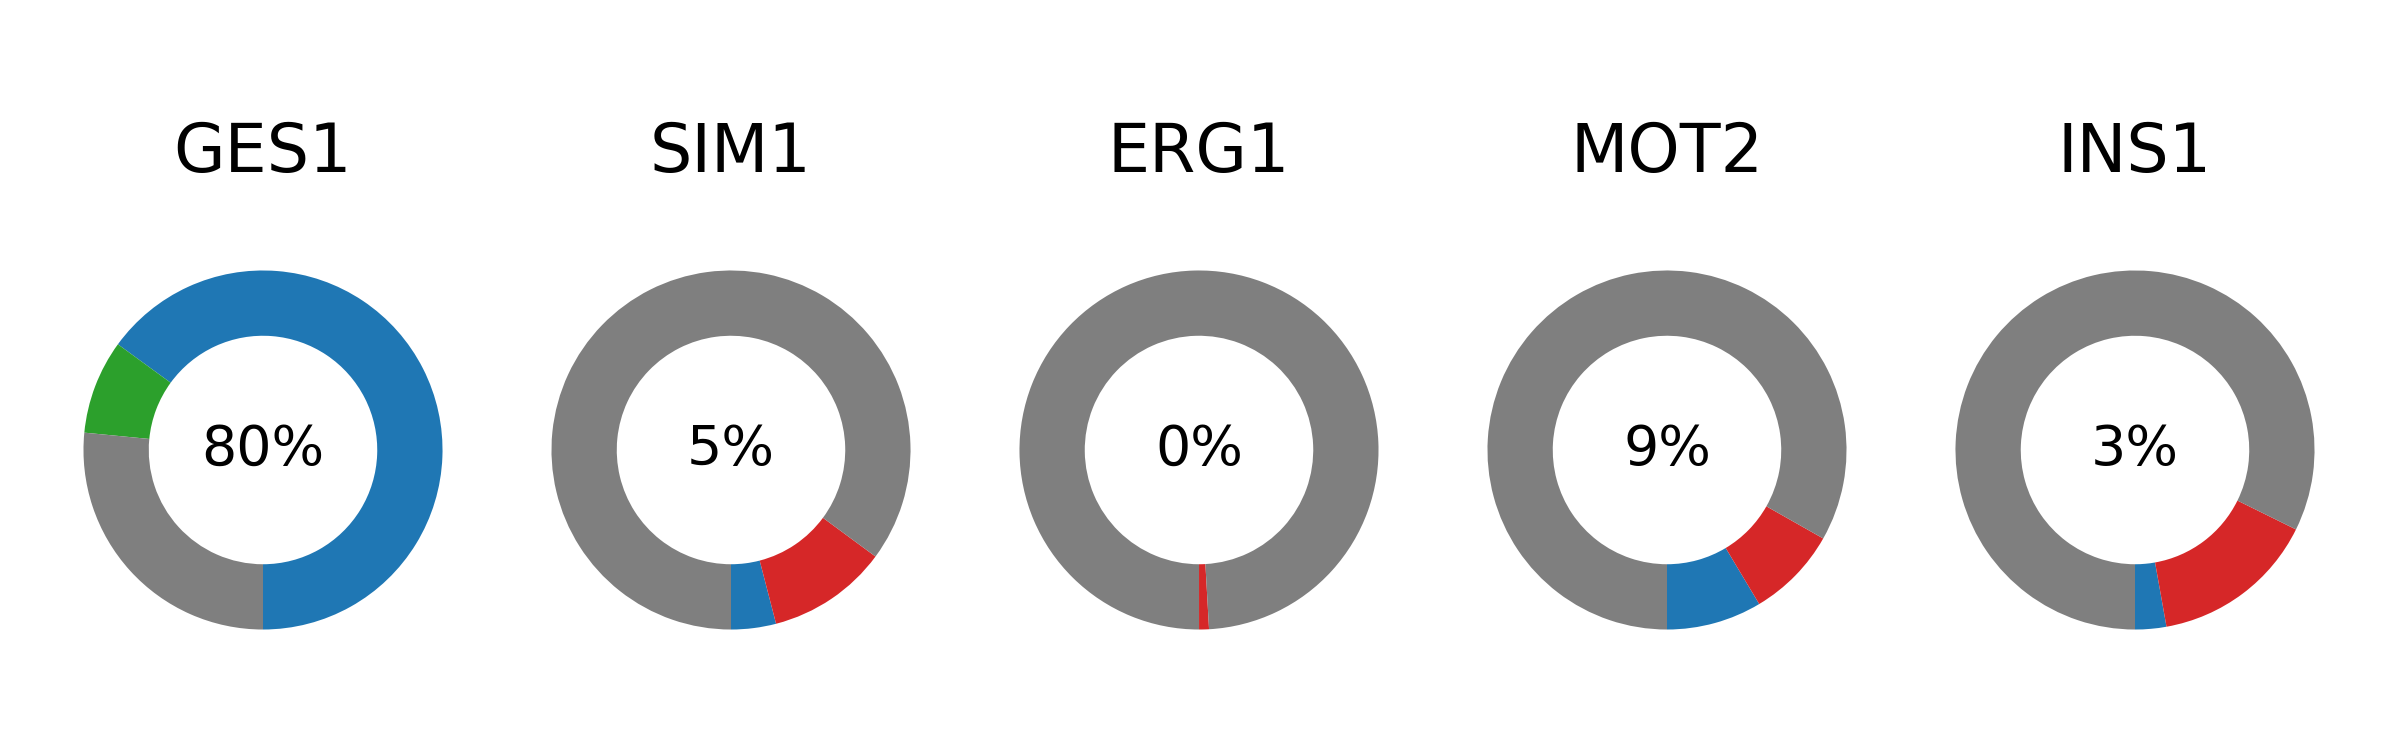
\includegraphics[width=.75\linewidth]{img/avancement.png}}

\vspace{0.2cm} % spacing vertical

}

% this states the box starts at column 0 (edge of page), directly below the box labelled subtopic1 for a span of 1 (column wide)

\headerbox{Problèmes}{name=problemes,column=0,below=taches,span=1}{

\vspace{.65cm}
\begin{itemize}
    \item \textbf{Faire un schéma de dataflow du simulateur:} Mauvais compréhension du flow de données du simulateur dans l'équipe informatique				
    \item \textbf{Peux pas entrer les heures dans le DVP:} Courbe en S est pas représentative.	
    \end{itemize}

    \vspace{1.8cm} % spacing vertical

}




\headerbox{Risques}{name=risques,column=0,span=3,below=problemes}{
{
    {
        \hspace{1cm}
        \centering
    	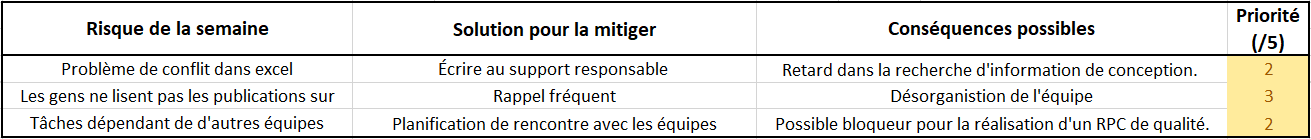
\includegraphics[scale=.46]{img/risques.png}
    }
}

}

\headerbox{Objectifs semaine prochaine}{name=objectifs_prochain,column=2,span=1,below=risques}{
{
    \vspace{.65cm}
    \begin{itemize}
    \item \textbf{Simulateur :}
    \begin{enumerate}
        \item Implémenter une V2 du simulateur
        \item Début programmation du dashboard
    \end{enumerate}
    \item \textbf{Contrôle :}
    \begin{enumerate}
        \item Faire des recherches sur le F.O.C, algorithmes de contrôle avec des inputs de plusieurs capteurs
    \end{enumerate}
    \item \textbf{Télémérie :}
    \begin{enumerate}
        \item Synchronisation avec les autres équipes pour la liste des capteurs					
    \end{enumerate}
    \item \textbf{Gestion et Documentation :}
    \begin{enumerate}
        \item Finir l'automatisation du tableau de bord
        \item Finir de remplir le DVP	
    \end{enumerate}
    \end{itemize}
    
    \vspace{2.5cm} % spacing vertical
}

}

\headerbox{Cashflow}{name=cashflow,column=0,span=2,below=risques}{
{

    \vspace{.6cm} % spacing vertical
    {
        \hspace{1cm}
        \centering
    	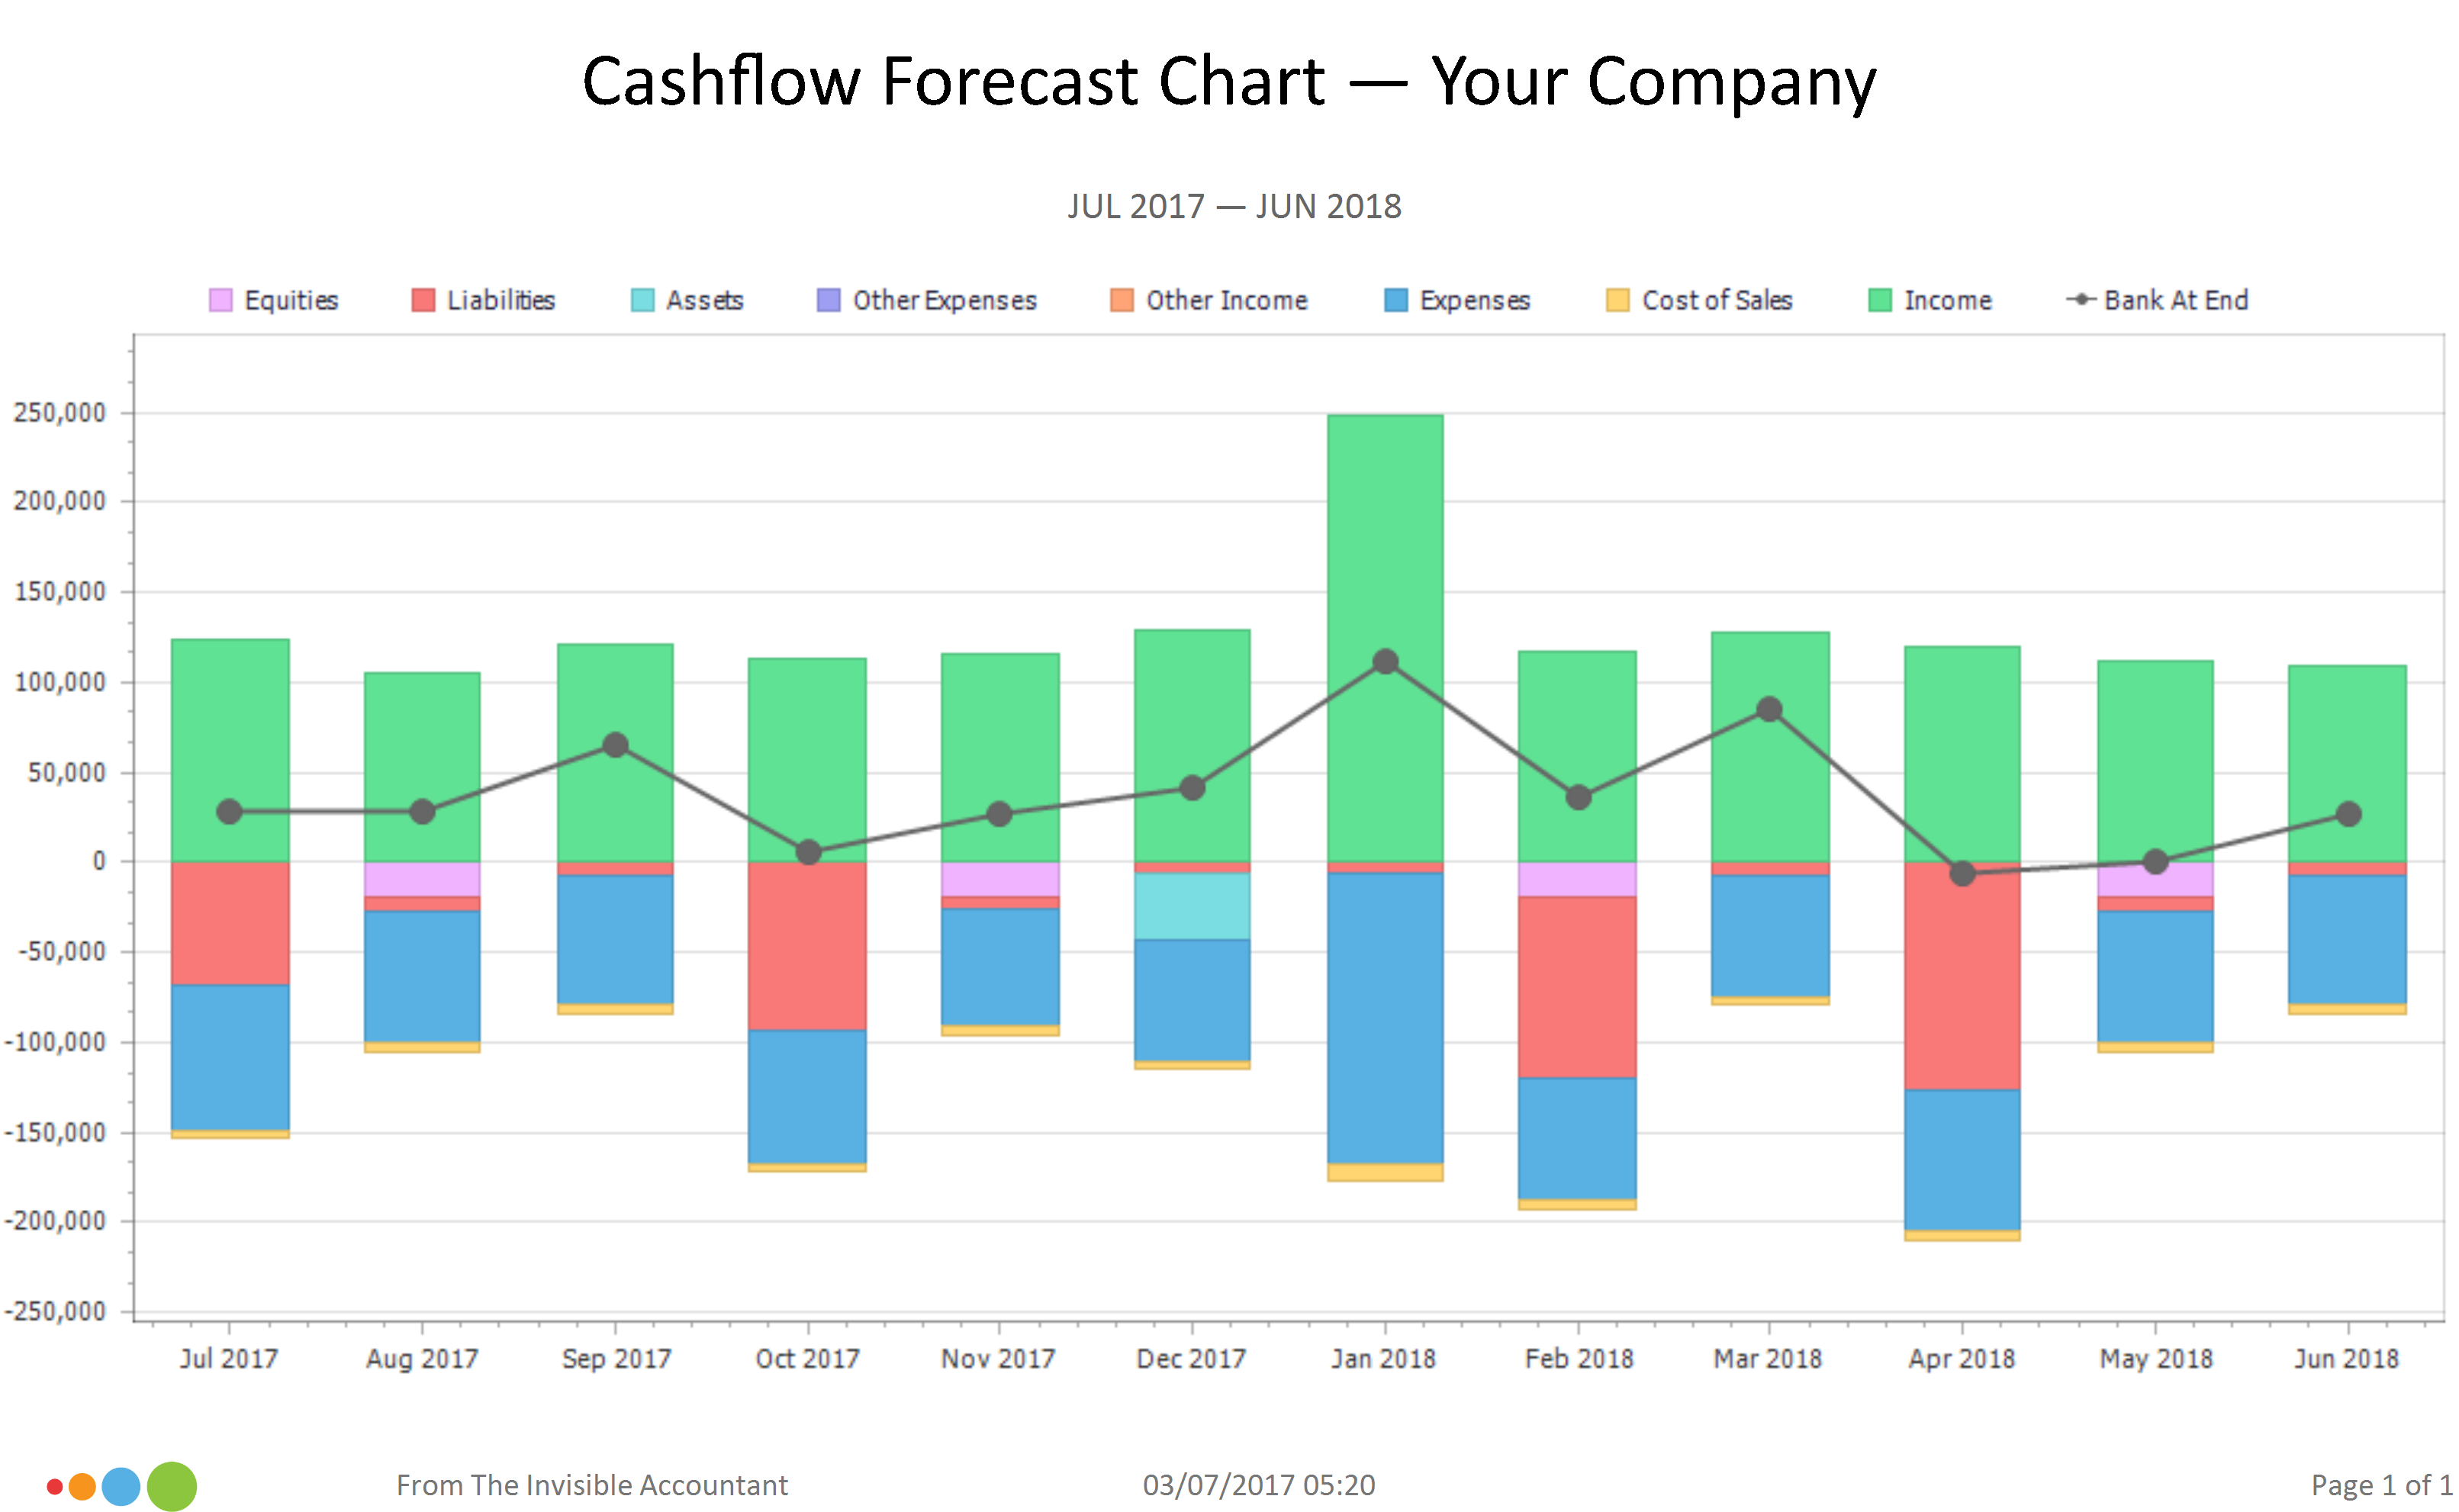
\includegraphics[scale=.5]{img/cashflow.png}
    }
    \vspace{1.15cm} % spacing vertical
}

}

\end{poster}




\end{document}
